\documentclass[a4paper]{article}

\usepackage{adjustbox}
\usepackage{algorithm}
\usepackage{algorithmic}
\usepackage{amsmath}
\usepackage{amssymb}
\usepackage{amsthm}
\usepackage{amsfonts}
\usepackage{afterpage}
\usepackage{blindtext}
\usepackage[font=footnotesize,labelfont=bf]{caption}
\usepackage{hyperref}
\usepackage[english]{babel}
\usepackage{bbm}
\usepackage{bigints}
\usepackage{bm}
\usepackage{cite}
\usepackage{color}
\usepackage{float}
\usepackage[left=2cm,right=2cm,top=2cm,bottom=2cm]{geometry}
\usepackage{graphicx}
\usepackage[utf8]{inputenc}
\usepackage{mathtools}
\usepackage{mdframed}
\usepackage{pgfplots} 
\usepackage{subfigure}
\usepackage{stmaryrd}
\usepackage{textcomp}
\usepackage{tikz}
\usepackage{url}
\renewcommand{\proofname}{Proof}
\theoremstyle{plain}
\newtheorem{monTheoNumrote}{Théorème}[section] % Environnement numéroté en fonction de la section
\newtheorem*{monTheoNonNumerote}{Théorème}  % Environnement non numéroté
\newtheorem{The}{Theorem}[section]
\newtheorem*{The*}{Theorem}
\newtheorem{Prop}{Proposition}[section]
\newtheorem*{Prop*}{Proposition} 
\newtheorem{Cor}{Corollary}[section]
\newtheorem*{Cor*}{Corollary}
\newtheorem{Conj}{Conjecture}[section]
\newtheorem{Lem}{Lemma}[section]
\renewcommand{\qed}{\unskip\nobreak\quad\qedsymbol}%
\numberwithin{equation}{section} % Numérote les équations section.numéro.
\theoremstyle{definition}
\newtheorem{Def}{Definition}[section]
\newtheorem{Rem}{Remark}[section]
\newtheorem*{Rem*}{Remark}
\newtheorem*{Lem*}{Lemma}
\newtheorem{Que}{Question}
\newcommand{\enstq}[2]{\left\{#1\mathrel{}\middle|\mathrel{}#2\right\}}
\newcommand{\Lp}[2]{L^#1(#2)}
\newcommand{\Sob}[3]{W^{#1,#2}(#3)}
\newcommand{\Rd}[0]{\mathbb{R}^d}
\newcommand{\RN}[0]{\mathbb{R}^N}
\newcommand{\Rn}[0]{\mathbb{R}^n}
\newcommand{\norm}[1]{\left\|#1\right\|}
\newcommand{\sinc}[0]{\textup{sinc}}
\newcommand{\functionDef}[5]{\begin{array}{lllll}
#1 & : & #2 & \longrightarrow & #3 \\
 & & #4 & \longmapsto &\displaystyle #5 \\
\end{array}}
\newcommand{\Theautorefname}{Theorem}
\newcommand{\Propautorefname}{Proposition}
\newcommand{\Corautorefname}{Corollary}
\newcommand{\Lemautorefname}{Lemma}
\newcommand{\Defautorefname}{Definition}
\newcommand{\N}{\mathbb{N}}
\newcommand{\Z}{\mathbb{Z}}
\newcommand{\D}{\mathbb{D}}
\newcommand{\R}{\mathbb{R}}
\newcommand{\A}{\mathcal{A}_{a,b}}
\newcommand{\Crad}{C^\infty_{c,rad}(B)}
\newcommand{\Lrad}{L^2_{rad}(B)}
\newcommand{\Lradab}{L^2_{rad}(\mathcal{A}_{a,b})}
\newcommand{\duality}[2]{\left\langle #1,#2\right\rangle}
\newcommand{\Hrad}{H^1_{rad}(B)}
\newcommand{\Hzrad}{H^1_{0,rad}(B)}
\newcommand{\rmin}{\delta_{\min}}
\newcommand{\rmax}{\delta_{\max}}
\newcommand{\corr}{\gamma}
\newcommand{\question}[1]{\begin{Que} \ 
#1
\end{Que}}
\newcommand{\abs}[1]{\left\lvert #1 \right\rvert}
\newcommand{\CL}[2]{\textup{CL}\left(\enstq{#1}{#2}\right)}
\newcommand{\Script}[1]{`\texttt{#1}`}
\newcommand{\espace}{\text{ }\qquad} 
\newcommand{\loc}{\text{loc}}
\newcommand{\SL}{\textup{SL}\hspace{1.5pt}}
\newcommand{\DL}{\textup{DL}\hspace{1.5pt}}
\newcommand{\fp}{\underset{\varepsilon \to 0}{\textup{f.p.}}}
\newcommand{\scalProd}[2]{\left(#1|#2\right)}
\newcommand{\toDo}[1]{{\color{red}#1}}
\newcommand{\bs}[1]{\boldsymbol{#1}}
\newcommand{\varInRange}[4]{(#1_{#2})_{#3 \leq #2 \leq #4}}
\newcommand{\from}{\colon}
\newcommand{\Cinf}{C^{\infty}}
\newcommand{\isdef}{\mathrel{\mathop:}=}
\newcommand{\defis}{=\mathrel{\mathop:}}

\renewcommand{\algorithmicrequire}{\textbf{Inputs:}}
\renewcommand{\algorithmicensure}{\textbf{Outputs:}}

\pgfplotsset{compat=1.13}

\title{Preconditionning the Helmholtz problem on curved arcs in dimension 2}
\author{Fran\c{c}ois Alouges and Martin Averseng\footnote{CMAP, Ecole polytechnique, Route de Saclay, 91128 Palaiseau Cedex.}}
\begin{document}
\maketitle

\begin{abstract}
	We introduce new efficient preconditioners for the Helmholtz weighted single layer potential and hypersingular on open curves. Those preconditioners are in the form of square roots of local differential operators. 
\end{abstract}

\section*{Introduction}

The problem of preconditionning the linear systems coming from the discretization of first kind integral equations has received considerable attention since two decades roughly. Among the possible strategies are the so-called 
pseudo-differential preconditionner, whose analysis uses tools from pseudo-differential calculus \cite{christiansen2002preconditioner,levadoux2005proposition,antoine2007generalized,mclean1997preconditioning}. \toDo{Ai-je cité les bons articles ?}. Roughly speaking, if the original problem is written in the abstract way
\begin{equation}
	\mathcal{L}u=f\,,
	\label{eq1}
\end{equation}
the strategy consists in findind a suitable operator $\mathcal{K}$ such
that, when left mulitplying the (\ref{eq1}) by $\mathcal{K}$, one needs to solve
\begin{equation}
	\mathcal{K}\mathcal{L}u=\mathcal{K}f\,.	
\end{equation}
Now if $\mathcal{K}\mathcal{L}$ is a compact perturbation of the identity, the condition number of the discretized underlying
system is independant of the chosen size of the mesh, leading to optimal convergence rate of the numerical methods used to solve the system.

Several strategies, depending on the problem to solve have been studied in the literature \cite{} \toDo{Tu voulais mettre qqch ici ?} to propose such operators $\mathcal{K}$, that often turn out to be very effective in practice, when numerical applications are considered.
However, all the preceding results and theories are limited to smooth domains and very little is known when the integral equation 
is posed on domains with corners (in 2D), wedges or conical points (in 3D). One of the reason might be the fact that 
pseudo-differential calculus is difficult to generalize on such manifolds, and more problematic, the underlying operators
are difficult to analyze on such domains.

Nevertheless, a program similar to those given on smooth manifold was proposed a few years ago \cite{bruno2012second,jerez2012explicit,hiptmair2017closed} \toDo{autres à rajouter ?} who tackled the problem of preconditionning the first or second layer potential for Laplace or Helmholtz equation in dimension 2 or 3 but for very particular domains: a straight and then curved segment in 2D and a unit disc in 3D. \toDo{Je ne suis pas vraiment d'accord, ils disent à chaque fois que par perturbation compacte on peut traiter le cas non-flat.}

Here, we build preconditioners for the single-layer potential and the hypersingular operator, using ideas inspired by pseudo-differential theory. These preconditioners are in the form of the square root of local operators, in close analogy to \cite{antoine2007generalized}, and lead to a drastic reduction of the number of the iterations in the GMRES method \cite{saad1986gmres}. Since our aim is to generalize our ideas to more complex geometries, both in 2D and 3D we do not use the high order spectral methods available for this problem \cite{bruno2012second}, but rather introduce the simplest possible Galerkin method with piecewise polynomial functions. The only difference as compared to usual boundary element methods is the use of a weighted $L^2$ space as the underlying Hilbert space. This translates into numerical quadratures with a weight on the open arc, together with a slightly refined mesh towards the edges of the arc. As a result, our numerical method involves only minor modifications with respect to standard BEM, and thus, can be implemented easily. We show that the orders of convergence obtained are the same as those on smooth closed curves for piecewise polynomials. 
	
The paper is organized as follows: in the first section, we give an overview of the resolution of the Laplace and Helmholtz scattering problems by means of layer potentials on open arcs. We then define two family of spaces, $T^s$ and $U^s$ in the second section, that will be the basis of our pseudo-differential theory. We introduce a class of operators for which we are able to estimate the order. In the third section, we apply these new tools to the Laplace equation in the case of the unit segment, and give explicit inverses of the weighted layer potentials in terms of square roots of local operators. We then generalize our results to non-zero frequency and non-flat arc in the fourth section. The last section is dedicated to expose the numerical method. 

%	The remainder of the paper focuses on the numerical solution of the integral equations \eqref{dirichletIntEq} and \eqref{NeumannIntEq} using Galerkin finite elements. Though this will not lead to spectral convergence as when using trigonometric polynomial, we aim to generalize our method to cases where the eigenvectors of the operators are not explicitly known. In the first section, we treat the two equations corresponding to the case $k=0$ and when $\Gamma$ is the segment. We introduce the same rescaled operators as in \cite{bruno2012second}. We derive a simple preconditioner for both integral equation in the form of the square root of the differential operators \eqref{cheb1} and \eqref{cheb2}, and verify its efficiency on numerical experiments using Galerkin discretization with piecewise polynomial finite elements. In the next section, we treat the general case using standard compact perturbation arguments, leading to a new preconditioner. Numerical tests are again provided.

\toDo{Peaufiner l'intro}

Throughout this article, $C$ refers to a constant which specific value can change from line to line. 

\section{The scattering problem outside an open curve}

Let $\Gamma$ be a smooth non-intersecting open curve, and let $k \geq 0$ the wave number. We seek a solution of the problem
\begin{equation}
	-\Delta u - k^2 u = 0,  \text{ in } \R^2 \setminus \Gamma
	\label{Helmholtz}
\end{equation}
when one considers furthermore
\begin{itemize}
	\item Dirichlet or Neumann boundary conditions, namely
	\begin{equation}
	u = u_D, \text{ on } \Gamma
	\label{Dirichlet}
	\end{equation}
	or
	\begin{equation}
	\dfrac{\partial u}{\partial n} = u_N  \text{ on } \Gamma 
	\label{Neumann}
	\end{equation}
	respectively.
	\item Suitable decay at infinity, given by the Sommerfeld condition
	\begin{equation}
	\dfrac{\partial u}{\partial r} - iku = o\left(\frac{1}{\sqrt{r}}\right)
	\label{Sommerfeld}
	\end{equation}
	with $r=|x|$ for $x\in \mathbb{R}^2$.
\end{itemize}
In the preceding equation $n$ stands for a smooth unit normal vector to $\Gamma$.

Existence and uniqueness of solutions to the previous problems are guaranteed by the following theorem.
\begin{The}
	(see e.g. \cite{stephan1984augmented,wendland1990hypersingular,monch1996numerical}) Assume $u_D \in H^{1/2}(\Gamma)$, and $u_N \in H^{-1/2}(\Gamma)$. Then problems (\ref{Helmholtz},\ref{Dirichlet},\ref{Sommerfeld}) and (\ref{Helmholtz},\ref{Neumann},\ref{Sommerfeld}) both possess a unique solution $u \in H^1_\textup{loc}(\R^2 \setminus \Gamma)$, which is of class $C^{\infty}$ outside $\Gamma$. Near the edges of the screen $\Gamma$ $\lambda$ is unbounded:
	\[\lambda(x) = O\left(\frac{1}{\sqrt{d(x,\partial \Gamma)}}\right).\]
	Near an edge of the arc, $\mu$ is locally given by
	\[\mu(x) = C\sqrt{d(x,\partial \Gamma)} + \psi\]
	where $\psi \in \tilde{H}^{3/2}(\Gamma)$.
\end{The}

For the definition of Sobolev spaces on smooth open curves, we follow
\cite{mclean2000strongly} by considering any smooth closed curve $\tilde{\Gamma}$ containing $\Gamma$, and defining 
\[H^s(\Gamma) = \enstq{U_{|\Gamma}}{ U \in H^s(\tilde{\Gamma}) }.\]

Obviously, this definition does not depend on the particular choice of the closed curve $\tilde{\Gamma}$ containing $\Gamma$. Moreover,
\[\tilde{H}^s(\Gamma) = \enstq{u \in H^s(\Gamma)}{\tilde{u} \in H^s(\tilde{\Gamma})}\]
where $\tilde{u}$ denotes the extension by zero of $u$ on $\tilde{\Gamma}$.

\paragraph{Single-layer potential}  
We define the single-layer potential by
\begin{equation}
	\mathcal{S}_k\lambda(x) = \int_{\Gamma}G_k(x-y)\lambda(y)d\sigma(y)
	\label{defSk}
\end{equation}
	where $G_k$ is the Green's function defined by 
\begin{equation}
	\left\{
	\begin{aligned}
		G_0(z) &= -\dfrac{1}{2\pi} \ln \abs{z}, && \text{ if } k= 0,\\
		G_k(z) &= \frac{i}{4}H_0(k|z|), && \text{ if } k > 0,
	\end{aligned} 
	\right.
\end{equation} 
for $x\in \mathbb{R}^2\setminus \Gamma$. Here $H_0$ is the Hankel function of the first kind. 
The solution $u$ of the Dirichlet problem can be computed from (\ref{Helmholtz},\ref{Dirichlet},\ref{Sommerfeld}) as
\begin{equation}
	u = \mathcal{S}_k \lambda
\end{equation}
where $\lambda \in \tilde{H}^{-1/2}(\Gamma)$ is the unique solution to 
\begin{equation}
	S_k \lambda = u_D\,.
	\label{Sklambda}
\end{equation}
Here, $S_k \isdef \gamma \mathcal{S}_k$ where $\gamma$ is the trace operator on $\Gamma$. The operator $S_k$ maps continuously $\tilde{H}^{-1/2}(\Gamma)$ to $H^{1/2}(\Gamma)$.

\paragraph{Double-layer and hypersingular potentials}
Similarly, we introduce the double layer potential $\mathcal{D}_k$ by 
\[\mathcal{D}_k \mu(x) = \int_{\Gamma} n(y) \cdot \nabla G_k(x-y) \mu(y) d\sigma(y).\]
for any smooth function $\mu$ defined on $\gamma$.
The normal derivative of $\mathcal{D}_k\mu$ is continuous across $\Gamma$, allowing us to define the hypersingular operator $N_k = \partial_n \mathcal{D}_k$. This operator admits the representation for $x\in \Gamma$
\begin{equation}
	N_k \mu = \lim_{\varepsilon \to 0^+} \int_{\Gamma} n(y) \cdot \nabla G(x + \varepsilon n(x) - y) \mu(y) d\sigma(y).
	\label{defNk}
\end{equation}
The kernel of this operator has a non-integrable singularity, but numerical calculations are made possible by the following formula, valid for smooth functions $\mu$ and $\nu$ that vanish at the extremities of $\Gamma$: 
\begin{equation}
	\duality{N_k \mu}{\nu} = \int_{\Gamma\times \Gamma} G_k(x-y) \mu'(x) \nu'(y) - k^2 G_k(x,y) \mu(x) \nu(y) n(x) \cdot n(y) d\sigma(x) d\sigma(y)\,.
	\label{NkenfonctiondeSk}
\end{equation}
It is also known that $N_k$ maps $\tilde{H}^{1/2}(\Gamma)$ to $H^{-1/2}(\Gamma)$ continuously, and that the solution $u$ to the Neumann problem (\ref{Helmholtz},\ref{Neumann},\ref{Sommerfeld}) can be written as
\begin{equation}
	u = \mathcal{D}_k \mu
\end{equation}
where $\mu \in \tilde{H}^{1/2}(\Gamma)$ solves
\begin{equation}
	N_k \mu = u_N\,.
	\label{Nkmu}
\end{equation}  
	
	
\section{Analytical setting}
\label{sec:analyticalSetting}

In this section, we introduce a new analytical setting that will allow us to analyze the integral equations in a unified and simple framework.	We introduce the Chebyshev polynomials of first and second kinds, respectively given by 
\[T_n(x) = \cos(n \arccos(x)),\]
and 
\[U_n(x) = \dfrac{\sin((n+1) \arccos(x))}{\sqrt{1 - x^2}}\,.\]
Let $\omega$ the operator $u(x) \mapsto \omega(x)u(x)$ with $\omega(x) = \sqrt{1 - x^2}$. Moreover, let $\partial_x$ the derivation operator. The Chebyshev polynomials satisfy
the ordinary differential equations

\begin{eqnarray*}
	(1-x^2)T_n'' -xT_n' +n^2T_n =0\,\mbox{ and }(1-x^2)U_n'' -3xU_n' +n(n+2)U_n =0
\end{eqnarray*}
which can be rewritten under the form
\begin{eqnarray}
	(\omega\partial_x)^2 T_n &=& -n^2T_n\,, \label{cheb1}\\
	(\partial_x\omega)^2 U_n &=& -(n+1)^2U_n\, .\label{cheb2}
\end{eqnarray}
(Notice that by $(\partial_x\omega) f$ we mean $(\omega f)'$.)
As we shall see, the preceding equations are crucial in our analysis. 

\subsection{Spaces $T^s$ and $U^s$}

Both $T_n$ and $U_n$ are polynomials of degree $n$, and form orthogonal families respectively of the Hilbert spaces 
$$L^2_{\frac{1}{\omega}} \isdef \enstq{u \in L^1_\textup{loc}(-1,1)} {\int_{-1}^{1} \dfrac{f^2(x)}{\sqrt{1 - x^2} }dx< + \infty}$$
and 
$$L^2_{\omega} \isdef \enstq{u \in L^1_\textup{loc}(-1,1)} {\int_{-1}^{1} {f^2(x)}{\sqrt{1 - x^2} }dx< + \infty}.$$
We denote by $\duality{\cdot}{\cdot}_\frac{1}{\omega}$ and $\duality{\cdot}{\cdot}_\omega$ the inner products in $L^2_{\frac{1}{\omega}}$ and $L^2_{\omega}$ respectively.
The Chebyshev polynomials satisfy
\begin{equation}
	\int_{-1}^1  \dfrac{T_n(x)T_m(x)}{\sqrt{1 - x^2} }dx = \left\{
	\begin{array}{l}
	0 \mbox{ if } n\ne m\\
	\pi \mbox{ if } m=n=0\\
	\pi/2 \mbox{ otherwise}
	\end{array} 
	\right.
\end{equation}
and
\begin{equation}
	\int_{-1}^1  U_n(x)U_m(x)\sqrt{1 - x^2} dx = \left\{
	\begin{array}{l}
	0 \mbox{ if } n\ne m\\
	\pi/2 \mbox{ otherwise}
	\end{array} 
	\right.
\end{equation}
which provides us with the so-called Fourier-Chebyshev decomposition. Any
$u\in L^2_{\frac{1}{\omega}}$ can be decomposed through the first kind Chebyshev series 
\begin{equation}
	u(x) = \sum_{n=0}^{+\infty} \hat{u}_n T_n(x)
	\label{FCseries}
\end{equation}
where the Fourier-Chebyshev coefficients $\hat{u}_n$ are given by 
\[ \hat{u}_n \isdef \begin{cases}
\dfrac{2}{\pi}\displaystyle\int_{-1}^{1} \dfrac{u(x) T_n(x)}{\sqrt{1-x^2}}dx & \text{ if } n \neq 0\,,\\
\dfrac{1}{\pi}\displaystyle\int_{-1}^{1} \dfrac{u(x)}{\sqrt{1-x^2}}dx & \text{ otherwise,}\\
\end{cases}\]
and satisfy the Parseval equality
\[ \int_{-1}^{1} \frac{u^2(x)}{\sqrt{1-x^2}} dx =  \frac{\pi \hat{u}_0^2}{2} + \pi\sum_{n=1}^{+\infty}\hat{u}_n^2\,.\]
When $u$ is furthermore a smooth function, the series \eqref{FCseries} converges uniformly to $u$. Similarly, any 
function $v\in L^2_{\omega}$ can be decomposed along the $U_n$ as
\[ v(x) = \sum_{n=0}^{+\infty} \check{v}_n U_n(x)\]
where the coefficients $\check{v}_n$ are given by 
\[ \check{v}_n \isdef 
\dfrac{2}{\pi}\displaystyle\int_{-1}^{1} v(x) U_n(x)\sqrt{1-x^2}dx  \]
with the Parseval identity
\[ \int_{-1}^{1} v^2(x)\sqrt{1-x^2} dx =  \frac{\pi}{2} \sum_{n=0}^{+\infty}\check{v}_n^2\,.\]
The preceding analysis can be generalized to define Sobolev-like spaces. 
\begin{Def}
	For all $s \geq 0$, we may define 
	\[T^s = \enstq{ u \in L^2_\frac{1}{\omega}}{ \sum_{n=0}^{+\infty}(1+n^2)^s \hat{u}_n^2 < + \infty}.\]
	This is a Hilbert space for the scalar product
	\[\duality{u}{v}_{T^s} = \frac{\pi}{2}\hat{u}_0 \hat{v}_0 + \pi\sum_{n=1}^{+\infty}(1+n^2)^s\hat{u}_n \hat{v}_n.\]
	We also define a semi-norm 
	\[\abs{u}_{T^s} \isdef \sum_{n = 1}^{+ \infty}n^{2s} \abs{\hat{u}_n}^2.\]
	We denote by $T^{\infty}$ the Fr\'echet space $T^{\infty} \isdef \displaystyle\cap_{s \in \R} T^s$, and by $T^{-\infty}$ the set of continuous linear forms on $T^{\infty}$. For $l \in T^{-\infty}$, we note $\hat{l}_n = l(T_n)$, so that for $u \in T^{\infty}$, 
	\[l(u) = \frac{\pi}{2}\hat{l}_0 \hat{u}_0 + \pi \sum_{n=1}^{+\infty} \hat{l}_n \hat{u}_n\,.\] 
	
	We choose to identify the dual of $L^2_\frac{1}{\omega}$ to itself using the previous bilinear form.  With this identification, any element of $T^s$ with $s \geq 0$ can also be seen as an element of $T^{-\infty}$.  
	Furthermore, the space $T^{-s}$ can be defined for all $s \geq 0$ as
	\[T^{-s} = \enstq{ u \in T^{-\infty}}{ \sum_{n=0}^{+\infty}{(1 + n^2)^{-s} \hat{u}_n^2} < \infty}.\]
	Using the former identification $T^{-s}$ becomes the dual of $T^s$. 
	For $s < t$, the inclusion $T^s \subset T^t$ is compact.
\end{Def}
\begin{Rem}
	The spaces $T^n$ correspond, up to a variable change, to the spaces $H^n_e$ defined in \cite{bruno2012second,atkinson1991numerical,yan1988integral,yan1990cosine} among other works, that is, the restriction of the usual Sobolev space $H^n$ to even periodic functions, as stated in \autoref{thmChar}.
\end{Rem}
\noindent In a similar fashion, we define the following spaces:
\begin{Def}
	For all $s \geq 0$, we set
	\[U^s = \enstq{u \in L^2_\omega}{ \sum_{n=0}^{+\infty} (1 + n^2)^s\check{u}_n^2}.\]
	We extend as before the definition to negative indices by setting $U^{-s}$ to be the dual of $U^s$ for $s\geq 0$, this time with respect to the duality $\duality{\cdot}{\cdot}_\omega$. 
\end{Def}
Obviously, for any real $s$, if $u \in T^s$ the sequence of polynomials 
\[S_N(x) = \sum_{n=0}^{N} \hat{u}_n T_n(x)\]
converges to $u$ in $T^s$. The same assertion holds for $u \in U^s$ when $T_n$ is replaced by $U_n$. Therefore
\begin{Lem}
	\label{densite}
	$C^{\infty}([-1,1])$ is dense in $T^s$ and $U^s$ for all $s \in \R$.
\end{Lem}
\noindent The polynomials $T_n$ and $U_n$ are connected by the following formulas:
\begin{equation}
\label{TnAsUn}
\forall n \geq 2, \quad T_n(x) = \frac{1}{2}\left(U_n - U_{n-2}\right),
\end{equation}
\begin{equation}
\label{UnAsTn}
\forall n \in \N, \quad U_{2n} = 2\sum_{j = 0}^n T_{2j} - 1, \quad U_{2n+1} = 2\sum_{j=0}^n T_{2j+1}.
\end{equation}

\begin{Lem}
	\label{inclusionsTsUs}
	For all real $s$, $T^s \subset U^s$ and for all $s > 1/2$, $U^s \subset T^{s-1}$.
\end{Lem}
\begin{proof}
	The first property is immediate from \eqref{TnAsUn}. 
	When $u \in U^{s}$ for $s > 1/2$, the series $\sum \abs{\check{u}_n}$ is converging, allowing to identify $u$ to a function in $T^{-\infty}$, with, in view of \eqref{UnAsTn}, 
	\[\hat{u}_{0} = \sum_{n=0}^{+ \infty} \check{u}_{2n}, \quad  \hat{u}_j = 2\sum_{n=0}^{+\infty} \check{u}_{j + 2n} \textup{ for } j \geq 1.\]
	Since $u \in U^s$, $(1+n^2)^{s/2} \abs{\check{u}}$ is in $l^2$ and by continuity of the adjoint of the Cesàro operator in $l^2$, the sequence $r_n \isdef \left( \sum_{k=n}^{+ \infty} (1+k^2)^{\frac{s-1}{2}} \abs{\check{u}_k}\right)_n$ is in $l^2$. But
	\begin{eqnarray*}
		\norm{u}_{T^{s-1}}^2 &=& \sum_{n=0}^{+ \infty} (1 + n^2)^{s-1} \abs{\hat{u}_n}^2\\ 
		&\leq& 4\sum_{n=0}^{+\infty}(1+n^2)^{s-1} \left(\sum_{k=n}^{+\infty} \abs{\check{u}_k}\right)^2 \\
		&\leq& 4\sum_{n=0}^{+ \infty}\left(\sum_{k=n}^{+\infty}(1+k^2)^{\frac{s-1}{2}} \abs{\check{u}_k})\right)^2.\\
		&=& 4\norm{r_n}^2_{l^2}.
	\end{eqnarray*}	
\end{proof}
One immediate consequence is that $T^{\infty} = U^{\infty}$.  Moreover, we have the following result:
\begin{Lem}
	\[T^{\infty} = C^{\infty}([-1,1])\,.\]
	\label{LemTinfCinf}
\end{Lem}
\begin{proof}
	If $u \in C^{\infty}([-1,1])$, then we can obtain by induction using integration by parts and \eqref{cheb1}, that for any $k \in \N$
	\[\hat{u}_n = \frac{(-1)^k}{n^{2k}} \int_{-1}^{1} \dfrac{(\omega\partial_x)^{2k} u(x) T_n(x)}{\omega(x)}dx.\]
	Noting that $(\omega \partial_x)^2 = (1-x^2)\partial_x^2 - x \partial_ x$, this proves that $C^{\infty}([-1,1]) \subset T^{\infty}$. 
	
	To prove the converse inclusion, first notice that, by normal convergence of the series, $T^{\infty} \subset C^0([-1,1]) $. Now, let $u \in T^{\infty}$, it suffices to show that $u' \in T^{\infty}$ and apply an induction argument. Applying term by term differentiation, we obtain
	\[u'(x) = \sum_{n=1}^{+\infty} n u_n U_{n-1}(x).\] 
	Therefore, $u'$ is in $U^{\infty} = T^{\infty}$. 
\end{proof}
\begin{Lem}
	\label{LemInjectionsContinues}
	For all $\varepsilon >0$, if $u \in T^{\frac{1}{2} + \varepsilon}$, then $u$ is continuous and there exists a constant $C$ such that for all $x \in [-1,1]$,
	\[ \abs{u(x)} \leq C \norm{u}_{T^{1/2 + \varepsilon}}.\]	
	Similarly, if $u \in U^{3/2 + \varepsilon}$, then $u$ is continuous and 
	\[ \abs{u(x)} \leq C \norm{u}_{U^{3/2 + \varepsilon}}.\]
\end{Lem}
\begin{proof}
	We write 
	\[\abs{u(x)} \leq \sum_{n = 0}^{+ \infty} \abs{\hat{u}_n}\]
	since for all $n$, $\norm{T_n}_{L^\infty} = 1$. Cauchy-Schwarz's inequality then yields
	\[\abs{u(x)} \leq \sqrt{\sum_{n= 0}^{+ \infty} \frac{1}{(1+ n^2)^{\frac{1}{2}+ \varepsilon}}} \norm{u}_{T^{\frac{1}{2} + \varepsilon}}.\]
	For the second statement, we use the inclusion $U^{s} \subset T^{s-1}$ valid for $s > 1/2$, as established in \autoref{inclusionsTsUs}. 
\end{proof}	
\begin{Lem}
	We have $L^2_\omega = \frac{1}{\omega}L^2_\frac{1}{\omega}$ and the pointwise multiplication by $\frac{1}{\omega}$ defines an bijective isometry from $L^2_\frac{1}{\omega}$ to $L^2_\omega$ with inverse $\omega$. 
	\label{isometrie}
\end{Lem}
\begin{Lem}
	\label{omega2continuUsTs}
	The multiplication by $\omega^2$ defines a continuous operator from $U^s$ to $T^s$. 
\end{Lem}
\begin{proof}
	This fact is a consequence of the identity $\omega^2 U_n = \frac{T_{n+2} - T_{n}}{2}$. 
\end{proof}
\begin{Lem}
	\label{derivations}
	For all real $s$, the operator $\partial_x$ can be extended into a continuous map from $T^{s+1}$ to $U^{s}$ as
	\[ \duality{\partial_x u}{v}_{\omega} \isdef -\duality{u}{\omega \partial_x \omega v}_{\frac{1}{\omega}}.\] 
	For all real $s$, the  operator $\omega \partial_x \omega$ can be extended into a continuous operator from $U^{s+1} \to T^{s}$ as
	\[\duality{\omega \partial_x \omega u}{v}_\frac{1}{\omega} \isdef -\duality{u}{\partial_x v}_\omega.\]
	
\end{Lem}
\begin{proof}
	First, note that if $v \in T^{\infty}$, then  $\omega \partial_x \omega v = (1-x^2)v' - xv \in T^{\infty}$. The definition of $\partial_x$ is thus correct. The claimed continuity  is an immediate consequence of 
	\[\omega \partial_x \omega U_n = -(n+1) T_{n+1}.\]
	The second assertion comes from $T_n' = nU_{n-1}$. 
\end{proof}
Contrary to intuition, the operator $\partial_x$ isn't continuous from $T^s$ to $T^{s-1}$. However, the following result holds:
\begin{Cor}
	\label{corDxT2T0}
	The operator $\partial_x$ is continuous from $T^{s+2}$ to $T^s$ for all $s > -1/2 $ and from $U^{s+2}$ to $U^s$ for all $s > - 3/2$.
\end{Cor}
\begin{proof}
	For the first case we use $\partial_x$ is continuous from $T^{s+2}$ to $U^{s+1}$ and then the identity is continuous from $U^{s+1}$ to $T^s$. For the second, we use the same arguments in the reverse order. 
\end{proof}
\begin{Lem}
	\label{omegadxetdxomga}
	The operator $\omega \partial_x$ defined on $T^{\infty}$ as 
	\[\omega \partial_x u = \omega u'\]
	has a continuous extension from $T^1$ to $T^0$. Similarly, the operator $\partial_x \omega$ has a continuous extension from $U^1$ to $U^0$. 
\end{Lem}
\begin{proof}
	For the first part, we use the fact that $\partial_x$ is continuous from $T^1$ to $U^0$, and, by \autoref{isometrie}, $\omega$ is continuous from $U^0$ to $T^0$. 
	For the second part, we use the fact that $\omega \partial_x \omega$ is continuous from $U^1$ to $T^0$, and from the same lemma, the multiplication by $\frac{1}{\omega}$ is continuous from $T^0$ to $U^0$. 
\end{proof}
We can now provide a characterization of the spaces $T^s$ and $U^s$ in terms of $L^2$ norms of the derivatives. For a function $u$ defined on $[a,b]$, we denote by $\tilde{u}$ the function defined on $[\theta_a,\theta_b] \isdef [\arccos(a),\arccos(b)]$ as
\[ \tilde{u}(\theta) = u(\cos(\theta))\]
and by $Vu$ the function defined as 
\[Vu(\theta) \isdef \sin(\theta) \tilde{u}(\theta).\]
\begin{Lem}
	A function $u$ belongs to the space $T^n$ if and only if $u = \tilde{u} \circ \arccos$ for some even function $\tilde{u}$ satisfying $\tilde{u}\in H^n(-\pi,\pi)$. In this case, 
	\[ \norm{u}_{T_n}\sim \norm{\tilde{u}}_{H^n}, \abs{u}_{T^n} \sim \abs{\tilde{u}}_{H^n}.\]
	Similarly, $u$ belongs to  $\in U^n$ if and only if $ u = \frac{1}{\sqrt{1 - x^2}} Vu  \circ  \arccos$  for some odd function $Vu$ in  $H^n(-\pi,\pi)$. In this case, 
	\[\norm{u}_{U_n} \sim \abs{Vu}_{H^n}.\]	
	Moreover, if $ u \in T^n$, then $(\omega \partial_x)^n u$ is in $L^2_\frac{1}{\omega}$ and 
	\[ \abs{u}_{T^n}^2 \sim \int_{-1}^{1} \frac{((\omega \partial_x)^n u)^2}{\omega}.\]
	\noindent If $u \in U^n$, then $(\partial_x \omega)^n u \in L^2_\omega$ and 
	\[ \norm{u}_{U_n} = \int_{-1}^{1}\omega ((\partial_x \omega)^n u)^2.\]
	\label{thmChar}
\end{Lem}
\begin{proof}
	The first two equivalences stem from the fact that 
	\[\hat{u}_n = \frac{1}{\pi}\int_{-\pi}^{\pi} \tilde{u}(\theta) \cos(n \theta), \quad  \check{u}_n = \frac{1}{\pi} \int_{-\pi}^{\pi} Vu(\theta) \sin((n+1)\theta)d\theta,\]
	which can be verified by using the change of variables $x = \cos\theta$ in the definitions of $\hat{u}_n$ and $\check{u}_n$. 
	Now, let us show that if $ u \in T^n$, then $(\omega \partial_x)^n$ is in $L^2_\frac{1}{\omega}$. The operator $(\omega \partial_x)^2$ is continuous from $T^s$ to $T^{s-2}$ for all real $s$ which implies the result if $n$ is even. If $n$ is odd, say $n = 2k + 1$, we write $(\omega \partial_x)((\omega \partial_x)^{2})^k$, and conclude using \autoref{omegadxetdxomga}.
	The same kind of proof also shows that if $u \in U^n$, $(\partial_x \omega )^nu \in L^2_\omega$.
	The rest of the proof can be performed by computing the quantities for functions in $C^{\infty}([-1,1])$, performing integrations by part and concluding with the density of $T^{\infty}$ in $T^s$ and $U^s$. 
\end{proof}
\subsection{Classes of operators on $T^s$}
\label{subsec:classesOfOp}
We now proceed to define a class of operators on $T^s$ that is stable under composition and enjoys some properties similar to pseudo-differential operators. However, we shall not look for asymptotic expansions of symbols, to keep matters as simple as possible. The class we define may thus be quite far from a proper definition of pseudo-differential operators. The main result we need is \autoref{CommutPDO}. To ease the computations, we define $T_n = T_{\abs{n}}$ for $n \in \Z$. 

\begin{Def}
	Let $p\in \R$. If  $A : T^{\infty} \to T^{-\infty}$ can be extended into a continuous operator from $T^{s}$ to $T^{s + p}$ for any $s \in \R$, we shall say that it is of order $p$ in the scale $T^s$. When an operator is of order $p$ for all $p \in \N$, we call it a smoothing operator. 
	
	An operator $A : U^{\infty} \to U^{-\infty}$ which maps continuously $U^s$ to $U^{s+p}$ for all real $s$ is said to be of order $p$ in the scale $U^s$. When the family ($U^s$ or $T^s$) is clear from the context, we simply say that $A$ is of order $p$. 
\end{Def}

\begin{Def}
	\label{DefEquivModTp}
	Let $A$ and $B$ to operators of order $s$ in the scale $T^s$. When the operator 
	$A - B$ is of order $p \in (0,+\infty]$, we shall write 
	\[A = B + T_p.\]
	When the scale is $U^s$ instead of $T^s$, we write 
	\[A = B + U_p.\]
\end{Def}

\begin{Def}
	For any real $p$, an operator $A$ belongs to the class $S^{p}$ if there exists a function $a : \N^2 \to \R$ satisfying: 
	\begin{itemize} 
		\item[(i)]$	\forall k \in \Z, \quad A T_k = \displaystyle\sum_{i = -\infty}^{+\infty} a(k,i)T_{k-i}$
		\item[(ii)]$	\forall \alpha \in \N, \forall  i,k  \in \Z, \quad  \abs{\Delta_k^\alpha a(k,i)} \leq C_{\alpha,i} (1 + k^2)^{p - \alpha}$
		\item[(iii)] There exists $N \in \N$ such that
		\[\abs{i} \geq N \implies \forall k \in \Z, \quad a(k,i) = 0.\]  
	\end{itemize}
	The function $a$ is called the symbol of $A$ and is denoted by $\sigma_A$. 
\end{Def}
\begin{Rem}
	The condition (i) does not define uniquely the symbol of $A$, since $T_{-n} = T_n$. We will not tackle the question whether conditions (ii) and (iii) ensure uniqueness. The notation $\sigma_A$ thus refers to one possible symbol of $A$. The symbols can be viewed as infinite matrix with a finite band of diagonals. Condition (ii) further requires that the coefficients on each diagonal be smooth functions of $k$. 
\end{Rem}
\begin{Lem}
	If $A\in S^p$, then $A$ is of order $p$ in the scale $T^s$. 
\end{Lem}
\begin{proof}
	Since the sum in the condition (i) is finite, by linearity, showing that the operator $A$ is of order $p$ amounts to proving that the operator $A_i$ defined by
	\[ \forall k \in \Z, \quad  A_i T_k = a(k,i) T_{k-i} \]
	is of order $p$. We treat the case $i > 0$, the opposite case being analogous. Let $u \in T^s$ for some $s$, there holds 
	\[ A_i u = \sum_{k = 0}^{+ \infty} a(k + i,i)\hat{u}_{k + i}T_k + \sum_{k = 0}^{i} a(i - k,i) \hat{u}_{i - k}T_k.\]
	Let $Vu$ and $Ru$ respectively the two terms of the rhs. Obviously, $R$ is a smoothing operator. Now, for all $k \in \N$ let
	\[\hat{v}_k \isdef a(i + k,i) \hat{u}_{i + k}.\]
	Applying Peetre's inequality, one has
	\[(1 + k^2)^{n + s}\abs{\hat{v}_k}^2 \leq C \left(1 + i^2\right)^{\abs{n + s}}\left(1 + (i + k)^2\right)^{n + s} \abs{a(k + i,i)}^2 \abs{\hat{u}_{k+i}}^2.\]
	Condition (ii) with $\alpha = 0$ yields
	\[\abs{a(k+i,i)}^2 \leq C\left(1 + (k+i)\right)^{-2n} \leq 2C \left(1 + (k+i)^2\right)^{-n}.\]
	Therefore, $\norm{V u}_{T^{s + n}} \leq C(1 + i)^{\abs{n + s}} \norm{u}_{T^s}$ which shows that $A$ is of order $p$.
\end{proof}
\begin{Lem}
	\label{LemCompo}
	If $A \in S^{p}$, $B \in S^{q}$, then $AB$ and $BA$ are in $S^{p + q}$, 
\end{Lem}
\begin{proof}
	The composition of two operators $A T_k = \sum_{i = -\infty}^{+ \infty} a(k,i) T_{k-i}$ and $B T_k = \sum_{i = - \infty}^{+ \infty} b(k,i) T_{k-i}$ gives rise to an operator $C = \sum_{i = - \infty}^{+ \infty} c(k,i) T_{k-i}$ for which a symbol is given by 
	\[c(k,i) = \sum_{j = - \infty}^{+ \infty} a(k - j, i - j) b(k,j).\]
	This formula is obtained writing the expression of $AB T_n$ using their symbol and using the identity $T_i T_j = T_{i + j} + T_{i -j}$. 
	The number of non-zero terms in this decomposition is obviously finite, so we must simply check the requirement (ii). It is enough to show that for any $j \in \Z$, the function $c_{i,j}(k) \isdef a(k-j,i-j) b(k,j)$ satisfies
	\[\forall \alpha \in \N, \forall i,k, \in \Z, \abs{\Delta_k^\alpha c_{i,j}} \leq C_{i,j,k} (1 + k^2)^{p + q - \alpha}.\]
	To prove this, one can check by induction that for any two functions $c,d : \N \to \R$, $\Delta^\alpha (c d)(k)$ is a linear combination of terms of the form $\Delta^\beta c(k_1) \Delta^{\alpha-\beta} d(k_2)$, where $k_1$ and $k_2$ lie in the interval $[k,k-\alpha]$. The conclusion follows after applying asumption (ii) for $A$ and $B$ and applying Peetre's inequality to the terms $(1 + (k_1)^2)^{p + \beta} (1 + (k_2)^2)^{q + \alpha - \beta}$. 
	and apply asumption (ii) for $A$ and $B$. 
\end{proof}
\begin{Lem}
	If $A \in S^{p}$ and $B \in S^q$, the $AB - BA$ is in $S^{p + q -1}$. 
	\label{CommutPDO}
\end{Lem}
\begin{proof}
	A symbol of $AB - BA$ is given by
	\[\sigma_{AB - BA}(k,i) = \sum_{j = -\infty}^{+\infty} a(k-j,i-j)b(k,j) - \sum_{j = - \infty}^{+\infty} b(k-j,i-j) a(k,j).\]
	In the second sum, we change the index to $j' = i -j$, yielding 
	\begin{eqnarray*}
		\sigma_{AB - BA}(k,i) &=& \sum_{j = -\infty}^{+\infty} a(k-j,i-j)b(k,j) - \sum_{j = - \infty}^{+\infty} b(k-i +j',j') a(k,i-j').\\
		&=& \sum_{j = -\infty}^{+\infty} \left[a(k-j,i-j) - a(k,i-j)\right]b(k,j) \\
		&& - \sum_{j = - \infty}^{+\infty} a(k,i-j) \left[b(k - i + j') -b(k,j)\right].\\
	\end{eqnarray*}
 	We show that asumption (ii) holds for one of the terms $\left[ a(k-j,i-j) - a(k,i-j)\right]b(k,j)$ when $j$ is positive. The other cases are treated analogously. We can write 
\begin{eqnarray*}
	a(k-j,i-j) - a(k,i-j) &=& \sum_{l = 0}^{j-1} a(k-j + l,i-j) - a(k-j + l +  1,i-j)\\
	&=& - \sum_{l = 0}^{j-1} \Delta a(k-j + l+1,i-j).
\end{eqnarray*}
The result then follows from the same considerations as in the proof of the previous result. 
\end{proof}
\begin{Lem}
	\label{lem:multPolyOrdre0}
	If $P$ is a polynomial, the multiplication by $P$ defines an operator of $S^0$. 
\end{Lem}
\begin{proof}
	For all $n$, we have $xT_n = \frac{T_{n+1} + T_{n-1}}{2}$, thus $x$ is in the class $S^0$. By \autoref{LemCompo}, the same is true for $x^n$ for any $n$, and by linearity, for any polynomial. 
\end{proof}
The next two lemmas enlarge the class of operators for which we can assess the order. \autoref{ordreNoyauxMultipl} allows us to treat a rather general class of operators and will allow us to evaluate the order of the remainders in Taylor expansions of the kernels. 
\begin{Lem}
	\label{lem:multByPsiOrdre0}
	If $\psi$ is a $C^{\infty}$ function on $[-1,1]$, then the operator
	\[ u(t) \mapsto \psi(t) u(t)\]
	is of order $0$, and for any $s \in \R$, 
	\[ \norm{\psi u}_{T^s} \leq C2^{\abs{s}/2}\norm{u}_{T^s} \norm{\psi}_{T^{\abs{s}+1}}.\]
	where $C$ is independent of $\psi$ and $s$. 
\end{Lem}
\begin{proof}
	Let $u \in T^s$, we rewrite $u$ as 
	\[ u = \sum_{n = -\infty}^{+ \infty}u_n'T_n\]
	where for $n< 0$ we define $T_{n} = T_{\abs{n}}$, and with 
	\[u_n' = \begin{cases}
	u_0 & \text{ if } n = 0\\
	\frac{u_{\abs{n}}}{2} & \text{ otherwise.}
	\end{cases}\]
	We apply the same idea to $\psi$, and using $T_m T_n = T_{m+n} + T_{m-n}$, 
	\[\psi u = \sum_{m,n} u'_n \psi'_m (T_{m+n} + T_{m-n}) = \sum_{m} \left(\sum_{n}u'_n(\psi'_{n + m} + \psi'_{n - m})\right) T_m\]
	that is, by parity
	\[\psi u = 2\sum_{m,n} u'_m \psi'_{m-n} T_{n}\]
	Using Peetre's inequality, we have 
	\[(1 + n^2)^{s/2}\abs{(\psi u)_n} \leq 2^{\abs{s}/2+1}\sum_{m}(1 + m^2)^{s/2} \abs{u'_m}  (1 + |n-m|^2)^{\abs{s/2}} \abs{\psi'_{n-m}} \]
	and by Young's inequality with $r = 2, p = 2, q = 1$, 
	\[\norm{\psi u}_s^2 \leq 2^{\abs{s}+2}\norm{u}_s^2 \sum_{m=-\infty}^{+\infty} (1 + m^2)^{\abs{s}/2}\abs{\psi'_m} \]		
	The last sum is finite because $\psi \in T^{\infty}$ and
	\[\sum_{m=-\infty}^{\infty}(1 + m^2)^{\abs{s}/2} \abs{\psi'_m} \leq \left(\sum_{m = -\infty}^{+ \infty} \frac{1}{1 + m^2} \right)\sum_{m=-\infty}^{+\infty} (1 + m^2)^{\abs{s}+1}\abs{\psi'}_m^2.\]
\end{proof}
\begin{Lem}
	\label{ordreNoyauxMultipl}
	Let $g(x,y)$ the kernel of an integral operator of order $\alpha \in \R$ in the spaces $T^s$, that is,
	\[G : u \mapsto \int_{-1}^{1} \frac{g(x,y) u(y)}{\omega(y)}dy\]
	is continuous from $T^s$ to $T^{s + \alpha}$ for all $s$. Let $R(x,y)$ a $C^{\infty}$ function. Then the operator 
	\[K : \int_{-1}^{1} \frac{g(x,y) R(x,y) u(y)}{\omega(y)}dy\]
	is of order $\alpha$. 
\end{Lem}
\begin{proof}
	Since $R$ is in $C^{\infty}$, one can show that $R$ admits the following expression:
	\begin{equation}
	R(x,y) = \sum_{m,n} r_{m,n} T_m(x) T_n(y)
	\label{sommenormalementcv}
	\end{equation}
	Moreover, the regularity of $R$ ensures $r_{m,n}$ satisfies for all $s,t \in \R$, 
	\[\sum_{m,n} (1 + m^2)^s (1 + n^2)^t\abs{r_{m,n}}^2 < +\infty.\] 
	To prove this property, one can for example apply the operator $(\omega \partial_x)^2$ repeatedly in the two variables. The resulting function is $C^\infty$, and in particular, square integrable on $[0,1] \times [0,1]$. We then write the Parseval's identity and the result follows. We can thus write 
	\[Ku = \sum_{m,n} r_{m,n} T_m G T_n u  \]
	where for each $m,n$, the operator $T_m G T_n$ is defined by 
	\[ T_m G T_n u (x)= T_m(x) \int_{-1}^{1} \dfrac{G(x,y) T_n(y)u(y)}{\omega(y)}dy.\]
	This operator is in $L(T^s,T^{s+\alpha})$ by the previous lemma, with 	
	\[\norm{T_m G T_n}_{T^s \to T^{s+\alpha}} \leq \norm{G}_{T^s \to T^{s + \alpha}} 2^{\abs{s} + \abs{s + \alpha}}(1 + n^2)^{\abs{s}+1}(1 + m^2)^{\abs{s+ \alpha} + 1}.\]
	thus, the series in \eqref{sommenormalementcv} is normally convergent in $L(T^s, T^{s + \alpha})$, which proves the claim. 
\end{proof}
In particular, when $g(x,y) \equiv 1$, $G$ is a smoothing operator thus
\begin{Cor}
	\label{lemSmoothingOp}
	Let $F \in C^{\infty}([-1,1]^2)$. Then
	\[ u \mapsto \int_{-1}^{1} \frac{F(x,y)u(y)}{\omega(y)}dy\]
	is a smoothing operator. 
\end{Cor}

\section{Laplace equation on a flat segment}

In this section, we restrict our attention to the case where $\Gamma$ is the open segment $(-1,1) \times \{0\}$, and $k=0$. We study the properties of the equations 
\[S\lambda = -u_D\]
and 
\[N\mu = u_N\]
and show their invertibility in a range of Sobolev-like spaces. This problem has been considered thoroughly, both
in terms of analytical and numerical properties in the literature (see for instance \cite{jiang2004second,bruno2012second}), and it turns out that the Chebyshev polynomials of first and second kind play a very important role. However, we go further compared to the literature by 
by constructing a functional framework close to Sobolev spaces, based on Chebyshev polynomials that
allows us to give a complete framework for the existence and uniqueness of the solutions to the preceding equations, as well as
new preconditioners.



\subsection{Single layer equation}

In this section we focus on the equation $S\lambda = g$, that is we seek $\lambda \in \tilde{H}^{-1/2}$ such that 
\begin{equation}
-\frac{1}{2\pi}\int_{-1}^{1} \log|x-y| \lambda(y) = -g(x), \quad \forall x\in (-1,1)\,.\label{Slambda}
\end{equation} 

This equation is sometimes called ``Symm's integral equation'' and its resolution has received a lot of attention in the 1990's. Numerical methods, using both collocation and Galerkin have been presented and analyzed \cite{atkinson1991numerical,yan1988integral,yan1990cosine,sloan1992collocation,yan1989mesh}. 

%The solution is connected to the exterior Dirichlet problem for the Laplace operator, but attention must be paid when the solution $\lambda$ obtained does not satisfy $\duality{1}{\lambda}_\Gamma = 0$: in this case, $\textup{SL}\lambda$ is not a bounded solution of the Dirichlet problem. See \cite{atkinson1991numerical} for a link with the logarithmic capacity of the line and how we recover the bounded solution from the solution of \eqref{Slambda}.

Our analysis lies on the following formula. For a proof, see for example \cite{mason2002chebyshev} Theorem 9.2. Note that this is also the main ingredient in several connected works, such as \cite{jiang2004second} and \cite{bruno2012second}.

%
%\paragraph{Autre idée de présentation.}
%We first start with a commutation result
%
%\toDo{Commencer par le truc connu. Et en fait c'est normal. Balancer ensuite la commutation. Dire que ça n'a pas été remarqué. }
%
%\begin{Prop}
%	Commutation de $S_\omega$ et $(\omega \partial_x)^2$. 
%\end{Prop}
%Exploitation en terme de vp. Dire qu'on a deux opérateurs avec spectre discret. (L'un est compact dans $L^2_\frac{1}{\omega}$, (sans preuve pour l'instant).
%
\begin{Lem}
	\[ -\frac{1}{2\pi}\int_{-1}^{1} \frac{\ln|x-y|}{\sqrt{1 - y^2}}T_n(y)dy = s_n T_n(x)\]
	where
	\[s_n = \begin{cases}
	\dfrac{\ln(2)}{2} & \text{if } n=0\\
	\dfrac{1}{2n} & \text{otherwise}.
	\end{cases}\]
	\label{STn}
\end{Lem}

Using the decomposition of $g$ and of the logarithmic kernel on the basis $T_n$, we see that the solution $\lambda$ to equation \eqref{Slambda} admits the following expansion 
\begin{equation}
\lambda(x) = \frac{1}{\sqrt{1-x^2}}\sum_{n=0}^{+ \infty} \frac{\hat{g}_n}{s_n} T_n(x).
\label{expansionLambda}
\end{equation}
We deduce the following well-known fact:
\begin{Cor}
	\label{CorSingularity}
	If the data $g$ is in $C^{\infty}([-1,1])$, the solution $\lambda$ to the equation 
	\[S\lambda = g\]
	is of the form 
	\[\lambda = \dfrac{\alpha}{\sqrt{1-x^2}}\]
	with $\alpha \in C^{\infty}([-1,1])$.  
	\begin{proof}
		Let $\alpha = \sqrt{1 - x^2}\lambda$ where $\lambda$ is the solution of $S\lambda = g$ with $g \in C^{\infty}([-1,1])$. 
		\autoref{LemTinfCinf} implies that $g \in T^{\infty}$, and by equation \eqref{expansionLambda}, 
		\[ \hat{\alpha}_n = \frac{\hat{g}_n}{s_n},\]
		so $\alpha$ also  belongs to $T^{\infty} = C^{\infty}([-1,1])$. 
	\end{proof}
\end{Cor}


We follow \cite{bruno2012second} by noticing that the behavior in $\frac{1}{\sqrt{1-x^2}}$ is consistent with the expected singularity near the edges and introduce the weighted single layer operator as the operator that appeared in Proposition \ref{STn}.
\begin{Def}(See \cite{bruno2012second}) 
	Let $S_\omega$ be the weighted single layer operator defined by
	\[\opFromTo{S_\omega}{\alpha \in \Cinf([-1,1])}{-\dfrac{1}{2\pi}}{\int_{-1}^1\dfrac{\ln|x-y|}{\omega(y)} \alpha(y)dy}\]
\end{Def}
\noindent We also recall that the operator $(\omega\partial_x)^2$ is defined by \[\opFromTo{(\omega\partial_x)^2}{\alpha \in \Cinf([-1,1])}{(1-x^2)\alpha''(x) - x \alpha'(x)}.\]

The action of these operators on $T^{\infty}$ is easy to analyze using \eqref{cheb1} and \autoref{STn}. By density of $T^{\infty}$ in $T^s$ for all $s$, we get:
\begin{Prop}
	The operator $S_\omega$ is a self-adjoint, positive definite operator, and defines a continuous bijection from $T^{s}$ to $T^{s+1}$ for all real $s$. In particular, $S_\omega$ is of order $1$ and is compact in $T^s$. 
	Similarly, for any $s \in \R$, the operator $-(\omega \partial_x)^2$ is positive, self-adjoint, and of order $-2$. 
\end{Prop}
\begin{proof}
	It suffices to remark that if $u=\sum_{n=0}^\infty \hat{u}_n T_n \in T^s$, then
	\[S_\omega u = \frac{\ln(2)}{2} \hat{u}_0 T_0 +  \sum_{n=1}^\infty \frac{\hat{u}_n}{2n} T_n\]
	while
	\[-(\omega \partial_x)^2 u = \sum_{n=0}^\infty n^2\hat{u}_n T_n \,.\]
\end{proof}
\begin{Rem}
	Of course, $S_\omega$ is in the class $S^1$ defined in \autoref{subsec:classesOfOp}
\end{Rem}
\noindent To obtain the solution of \eqref{Slambda}, we can thus solve 
\begin{equation}
S_\omega \alpha = -u_D,
\label{Somegaalpha}
\end{equation}
and let $\lambda = \frac{\alpha}{\omega}$.  
The next lemmas make clear the connection between the spaces $T^s$ with $s = \pm \frac{1}{2}$ and the usual Sobolev spaces. Equivalent results are proved in \cite{jerez2010boundary}. 
\begin{Lem}
	\label{LemmaT-1/2}
	We have $\tilde{H}^{-1/2}(-1,1) = \frac{1}{\omega}T^{-1/2}$ and for all $u \in \tilde{H}^{-1/2}(-1,1)$,
	\[\norm{u}_{\tilde{H}^{-1/2}} \sim \norm{\omega u}_{T^{-1/2}}.\] 
\end{Lem}

\begin{proof}
	Since the logarithmic capacity of the segment is $\frac{1}{4}$, the operator $S$ is positive and bounded from below on $\tilde{H}^{-1/2}(-1,1)$, (see \cite{mclean2000strongly} chap. 8). Therefore the norm on $\tilde{H}^{-1/2}(-1,1)$ is equivalent to 
	\[\norm{u}_{\tilde{H}^{-1/2}} \sim \sqrt{\duality{Su}{u}}.\]
	On the other hand, it is obvious that if $\alpha\in T^{-1/2}$
	\[ \norm{\alpha}_{T^{-1/2}} \sim \sqrt{\duality{S_\omega \alpha}{\alpha}_\omega}.\]
	It remains to notice that for $\alpha=\omega u$, the two duality products coincide.
\end{proof}

\begin{Lem} Similarly,
	\[H^{1/2}(-1,1) = T^{1/2}\]
	and for $u \in H^{1/2}(-1,1)$ we have
	\[\norm{u}_{H^{1/2}} \sim \norm{u}_{T^{1/2}}\,.\]
	\label{LemmaT1/2}
\end{Lem}	
\begin{proof}
	We know that $(H^{1/2})'(-1,1) =  \tilde{H}^{-1/2}(-1,1)$ (cf \cite{mclean1986spectral} chap. 3), and therefore
	\[\norm{u}_{H^{\frac{1}{2}}} = \sup_{ v\neq 0} \dfrac{\duality{u}{v}}{\norm{v}_{\tilde{H}^{-\frac{1}{2}}}}\,.\]
	According to the previous lemma, for all $v\in \tilde{H}^{-\frac{1}{2}}$, the function $\alpha = \omega v$ is in $T^{-1/2}$, and $\norm{ v}_{\tilde{H}^{-1/2}} \sim \norm{\alpha}_{T^{-1/2}}$, while $\duality{u}{v} = \duality{u}{\alpha}_\omega$. Thus 
	\[\norm{u}_{H^{1/2}} \sim \sup_{\alpha \neq 0} \dfrac{\duality{u}{\alpha}_\omega}{\norm{\alpha}_{T^{-1/2}}}\]
	The last quantity is the $T^{1/2}$ norm of $u$ since $T^{1/2}$ is identified to the dual of $T^{-1/2}$ for $\duality{\cdot}{\cdot}_\omega$. 
\end{proof}

We are now in a position to find an expression for the inverse of $S_\omega$. An explicit inverse has already appeared in the literature. In 
particular, in \cite{jerez2012explicit,urzua2014optimal}, explicit variational forms for this inverse operator are derived rigorously. (A similar method is also employed in the recent paper \cite{hiptmair2017closed} in $\R^3$ for the case of the unit disk.) We just state here the following formal decomposition:
\[\dfrac{d^2}{dxdy}\log\frac{M(x,y)}{|x-y|^2} = \frac{-1+xy}{2|x-y|^2} = \sum_{n=1}^{+ \infty} n T_n(x)T_n(y)\]
with 
$M(x,y) = \frac{1}{2}\left((y-x)^2 + (\omega(x) + \omega(y))^2\right) $.

However, using the preceding analysis, we have an alternative way of defining this exact inverse, which leads to an expression in the form of the square root of a local operator. To state the next result, we define the operator $\pi_{0}$ as the $L^2_{1/\omega}$ 
orthogonal projector on $T_0$. Namely 
\[\pi_0 \alpha(x)  = \frac{1}{\pi} \int_{-1}^{1}\frac{\alpha(y)}{\omega(y)}dy\,.\]
The preceding definition can be extended to $u \in T^s$ for any $s \in \R$ by setting $\pi_0 u$ as the solution of
\[\left\{
\begin{array}{l}\duality{\alpha-\pi_0 \alpha}{T_0}_{\frac{1}{\omega}} = 0\,,\\
\pi_0\alpha\in \mbox{Span}(T_0)\,,
\end{array}
\right.\]
since $T_0\in T^\infty$. Of course, $\pi_0$ is continuous from $T^s$ to $T^{\infty}$ for any $s$. 

\begin{The}
	\label{TheSdx2S}
	There holds
	\begin{equation}
		\label{Sdx2S}
		S_{\omega}^2 = \frac{1}{4}\left(-(\omega\partial_x)^2 + \frac{1}{\ln(2)^2} \pi_0 \right)^{-1}\,.
	\end{equation}
\end{The}
\begin{proof}
	The Chebyshev polynomials $(T_n)$ are a common Hilbert basis of eigenvectors for the three operators $S_\omega$, $-(\omega \partial_x)^2$ and $\pi_0$, so it is sufficient to compute $4 S_\omega^2 \left(-(\omega\partial_x)^2 + \frac{1}{\ln(2)^2} \pi_0 \right) T_n$ and check that this is indeed equal to $T_n$. 
	One has using the explicit eigenvalues for $S_\omega$. This is easily verified using the following expressions
	\[ S_\omega T_n =\frac{1}{2n}T_n\,,\,\, \pi_0 T_n = 0 \mbox{ and } -(\omega\partial_x)^2T_n = n^2 T_n \mbox{ if } n\ne 0\,,\]
	while
	\[ S_\omega T_0 = \frac{\ln(2)}{2} T_0\,,\,\, \pi_0 T_0 = T_0 \mbox{ and } -(\omega\partial_x)^2T_0 = 0 \mbox{ otherwise.}\]
\end{proof}

From the preceding formula, we can extract the explicit inverse of $S_\omega$ in terms of the square root of the inner operator. 

\begin{Cor}
	The inverse of $S_\omega$ can be equivalently expressed as 
	\begin{equation}
	S_{\omega}^{-1} = 2\sqrt{-(\omega \partial_x)^2 + \frac{1}{\ln(2)^2}\pi_0}\,.
	\end{equation}
\end{Cor}

The last result shows that $\sqrt{-(\omega \partial_x)^2}$ and $S_\omega$ can be thought as inverse operators (modulo constant terms) and that, at the very least, $\sqrt{-(\omega \partial_x)^2}$ can be used as a preconditioner for $S_\omega$. Indeed, $2\sqrt{-(\omega \partial_x)^2}S_\omega$ is a compact perturbation of identity. This makes a clear link with the approximation of the Dirichlet to Neumann map proposed in \cite{antoine2007generalized} in terms of a square root operator. The link will be even clearer when Helmholtz equation will be considered. In \autoref{TableNitTimeLaplaceDirichlet}, we compare the number of iterations for the numerical resolution of Equation \eqref{Somegaalpha} by the method detailed in \autoref{sec:numerMeth} without preconditioner, and with a preconditioner given by $M^{-1} \left[B \right] M^{-1}$ where $M$ is the mass matrix and $\left[ B \right]$ is the Galerkin matrix of the operator $\sqrt{ -(\omega \partial_x)^2 + \frac{1}{\ln(2)^2} \pi_0}$. The right hand side in \eqref{Somegaalpha} is chosen as $u_D(x) = (x^2 + 0.001)^{-1/2}, x \in (-1,1)$.
	
\begin{table}[H]
	\begin{center}
		\begin{tabular}{|| m{4em} | m{4em} | m{4em} | m{4em} | m{4em}||} 
			\hline
			\multicolumn{1}{||c|}{ }&
			\multicolumn{2}{c|}{with Prec.}&\multicolumn{2}{c||}{without Prec.}\\
			\hline
			$N$ & $n_{it}$& t(s) & $n_{it}$ & t(s)\\
			\hline\hline
			50 & 7 & 0.11 & 35 & 0.21\\
			\hline
			200 & 7 & 0.14 & 53 & 0.55\\
			\hline
			800 & 7 & 0.29 & 76 & 2.0 \\
			\hline
			3200 & 7 & 0.95 & 107 & 9.5\\
			\hline
		\end{tabular}
	\end{center}
	\caption{Number of iteration and time needed for the numerical resolution of \eqref{Somegaalpha} using Galerkin finite elements with and without preconditioner.}
	\label{TableNitTimeLaplaceDirichlet}
\end{table}
\begin{figure}[H]
	\centering
	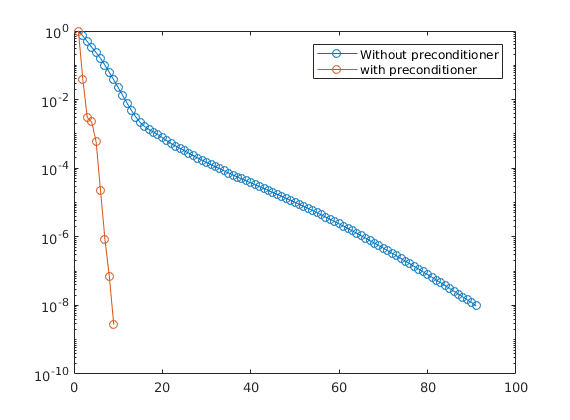
\includegraphics[scale=0.7]{figs/PrecondDirichletLaplaceSeg.png}
	\caption{Number of iteration in the resolution of the single layer integral equation with a mesh of size $N = 1600$.}
	\label{FigureNitLaplaceDirichlet}
\end{figure}

\subsection{Hypersingular equation} 

We now turn our attention to the equation 

\begin{equation}
N\mu = g
\label{Nmu}
\end{equation} 

Similarly to the previous section and following again the idea of \cite{bruno2012second}, we consider a rescaled version of the hypersingular operator $N_\omega \isdef N \omega$ defined by

\[N_\omega \mu = \lim_{\varepsilon\to 0}\int_{-1}^{1} n(y)\cdot\nabla G(x + \varepsilon n(x) - y) \sqrt{1-y^2} dy\]
We can get the solution to equation \eqref{Nmu} by solving 
\begin{equation}
N_\omega \beta = u_N,
\label{Nomegabeta}
\end{equation}
and letting $\mu = \omega \beta$. 
We now show that $N_\omega$ can also be analyzed in our functional framework, using this time the spaces $U^s$. 
\begin{Lem}
	\label{lemIPP}
	For any $\beta$, $\beta'$, one has 
	\[\duality{N_\omega \beta}{ \beta'}_\omega = \duality{S_\omega \omega \partial_x \omega \beta}{\omega \partial_x \omega \beta'}_\frac{1}{\omega}.\]
	\begin{proof}
		It is sufficient to show this formula for $\beta$ and $\beta'$ in $U^{\infty}$ by density. Indeed, for such $\beta, \beta'$, both sides of the identity define continuous bilinear forms on $T^{\infty}$. We use the well-known integration by part formula
		\[\duality{N u}{v} = \duality{S\partial_x u}{\partial_x v},\]
		valid when $u$ and $v$ vanish at the extremities of the segment (see for example \cite{bruno2012second}). 
		For a smooth $\beta$, we thus have
		\[ \duality{N (\omega \beta)}{ (\omega \beta')} = \duality{S \partial_x(\omega \beta)}{\partial_x (\omega \beta')}\] 
		which obviously implies the announced identity. 
	\end{proof}
\end{Lem}
\begin{Prop}
	$N_\omega$ is a positive definite, self-adjoint operator continuous from $U^s$ to $U^{s-1}$ for all real $s$. For all $n \in \N$, we have 
	\[N_\omega U_n = \frac{n+1}{2}U_n.\]
	Moreover, $-(\partial_x\omega)^2$ is also positive definite of order $2$.
	\label{NUn}
\end{Prop}
\begin{proof}
	From identity $T_{n+1}' = (n+1)U_n$ and Equation $\eqref{cheb1}$ we obtain
	\begin{equation*}
	\omega \partial_x \omega U_n = -(n+1) T_{n+1}.
	\end{equation*}
	Therefore, by \autoref{lemIPP}
	\begin{eqnarray*}
		\duality{N_\omega U_m}{U_n}_\omega & = & (n+1)(m+1)\duality{S_\omega T_{m+1}}{T_{n+1}}_\frac{1}{\omega}\\
		&=& \delta_{m=n} \frac{n+1}{2}.	
	\end{eqnarray*}
	The fact that $-(\partial_x \omega)^2$ is self-adjoint positive definite of order $2$ is a consequence of Equation \eqref{cheb2}.
\end{proof}
	Like before, we have the following link between $U^{-1/2}$, $U^{1/2}$ and the usual Sobolev spaces. 
\begin{Lem} The following identities hold, 
	\[\omega U^{1/2} = \tilde{H}^{1/2}(-1,1),\]
	\[ U^{-1/2} = H^{-1/2}(-1,1),\]
	with 
	\[\norm{\omega u}_{\tilde{H}^{1/2}} \sim \norm{u}_{U^{1/2}},\quad \norm{u}_{U^{-1/2}} \sim \norm{u}_{H^{-1/2}}.\]
	\label{lemU12H12}
\end{Lem}
\begin{proof} It suffices to remark that 
	\[ \norm{\omega u}_{\tilde{H}^{1/2}} \sim \sqrt{\duality{N\omega u}{\omega u}} = \sqrt{\duality{N_\omega u}{u}_\omega} \sim \norm{u}_{U^{1/2}}\,.\]
	The second equality follows from the same calculations that were done in Lemma \ref{LemmaT1/2},, as well as the norm equivalence. 
\end{proof}
As an application of this result, one can also derive the formal expansions as in \cite{jerez2012explicit}
\[\frac{1}{(x-y)^2} = \sum_{n=0}^{+\infty} 2(n+1)U_n(x)U_n(y)\,,\]
that lead, by applying for $(\partial_x\omega)^{-2}$ on both sides, to the following explicit kernel for the inverse of $N_\omega$:
\[\ln\left(\dfrac{(y-x)^2 + (\omega(x) + \omega(y))^2}{2|x-y|}\right) = \sum_{n=0}^{+\infty} \dfrac{2 U_n(x) U_n(y)}{n+1}.\]
Here instead, we give a simple expression of the inverse of $N_\omega$ as the inverse square root of a local operator:
\begin{The} 
	\label{the:NeumannInverseLaplace}
	There holds 
	\[N_\omega^2 = -\frac{1}{4}(\partial_x \omega)^2 \,.\]
	The inverse of $N_\omega$ is therefore 
	\begin{equation}
	N_\omega^{-1} = 2\sqrt{-(\partial_x \omega)^{-2}}\,.
	\end{equation}
\end{The}
In \autoref{TableNitTimeLaplaceNeumann}, we compare the number of iterations for the numerical resolution of Equation \eqref{Nomegabeta} by the method detailed in \autoref{sec:numerMeth} without preconditioner, and with a preconditioner given by $M^{-1} \left[B \right] M^{-1}$ where $M$ is the mass matrix and $\left[ B \right]$ is the Galerkin matrix of the operator $\sqrt{ -( \partial_x \omega)^{-2}}$. The right hand side in \eqref{Nomegabeta} is chosen as $u_N(x) = (x^2 + 0.001)^{1/2}, x \in (-1,1)$.

\begin{table}[H]
	\begin{center}
		\begin{tabular}{|| m{4em} | m{4em} | m{4em} | m{4em} | m{4em}||} 
			\hline
			\multicolumn{1}{||c|}{ }&
			\multicolumn{2}{c|}{with Prec.}&\multicolumn{2}{c||}{without Prec.}\\
			\hline
			$N$ & $n_{it}$& t(s) & $n_{it}$ & t(s)\\
			\hline\hline
			50 & 4 & 0.05 & 50 & 0.05\\
			\hline
			200 & 3 & 0.05 & 200 & 0.25\\
			\hline
			800 & 3 & 0.06 & 799 & 3.7 \\
			\hline
			3200 & 3 & 0.6 & 3007 & 630\\
			\hline
		\end{tabular}
	\end{center}
	\caption{Number of iteration and time needed for the numerical resolution of \eqref{Somegaalpha} using Galerkin finite elements with and without preconditioner.}
	\label{TableNitTimeLaplaceNeumann}
\end{table}
\begin{figure}[H]
	\centering
	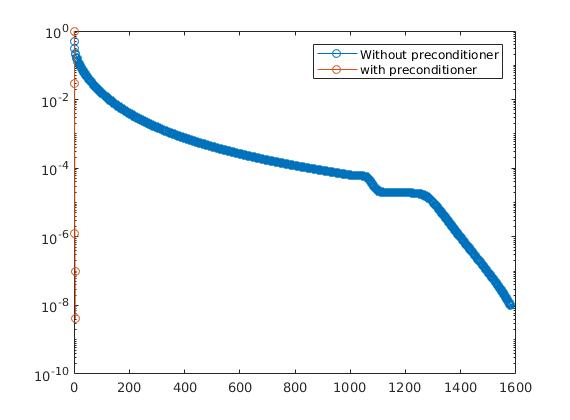
\includegraphics[scale=0.7]{figs/PrecondNeumannLaplaceSeg.png}
	\caption{Number of iteration in the resolution of the hypersingular  integral equation with a mesh of size $N = 1600$. The importance of preconditioning in this case is more obvious than in the case of the single-layer equation.}
	\label{FigureNitLaplaceNeumann}
\end{figure}

\begin{Rem}
	In \cite{bruno2012second}, the main theorem is equivalent to stating that $N_\omega S_\omega$ and $S_\omega N_\omega$ are bicontinuous operators in $T^s$, with a spectrum concentrated around $\frac{1}{4}$, which can be exploited for preconditioning purposes. It is shown that $N_\omega$ is continuous from $T^s$ to $T^{s-1}$ for all $s >1$ (in fact, this remains true for $s > \frac{1}{2}$). The two main arguments involved in the proof are the explicit expression of $N_\omega T_n$ and the continuity of the adjoint of the Cesaro operator in $l^2(\N)$. The same arguments can be used to prove that $S_\omega$ is also a bicontinuous operator from $U^s$ to $U^{s+1}$ for all $s > 1/2$. 
\end{Rem}



\section{Helmholtz equation}
	
	In this section, we introduce preconditioners for the integral equations on $\Gamma = (-1,1)$ for the Helmholtz equation. Recall the definition of the single layer and hypersingular operators, $S_k$ and $N_k$, given in \eqref{defSk} and \eqref{defNk}, and the integral equations for the Dirichlet and Neumann problems, \eqref{Sklambda} and \eqref{Nkmu}. As before, let $S_{k,\omega} \isdef S_k \frac{1}{\omega}$ and $N_{k,\omega} \isdef N_k \omega$. We begin by establishing the following result:
	
	\begin{The}
		\label{Commutations}
		The following commutations hold:
		\[S_{k,\omega} \left[-(\omega \partial_x)^2 - k^2\omega^2\right] =  \left[-(\omega \partial_x)^2 - k^2\omega^2\right]S_{k,\omega},\]
		\[N_{k,\omega} \left[-(\partial_x \omega)^2 - k^2\omega^2\right] =  \left[-(\partial_x \omega)^2 - k^2\omega^2\right]N_{k,\omega}.\]
		\begin{proof}
			We start with the first commutation. Since $(\omega \partial_x)^2$ is self adjoint and symmetric, we have 
			\[S_{k,\omega} (\omega \partial_x)^2 = \int_{-1}^{1} \frac{(\omega_y \partial_y)^2 \left[G_k(x-y)\right] u(y)}{\omega(y)},\]
			where we use the notation $\omega_y$ and $\partial_y$ to emphasize the dependence in the variable $y$. 
			Thus, 
			\[S_{k,\omega} (\omega \partial_x)^2 - (\omega \partial_x)^2 S_{k,\omega} = \int_{-1}^{1} \frac{D_k(x,y)u(y)}{\omega(y)},\]
			where $D_k(x,y) \isdef \left[(\omega_y \partial_y)^2 - (\omega_x \partial_x)^2\right] \left[G_k(x-y)\right]$. 
			One has 
			\[D_k(x,y) = G_k''(x-y) (\omega^2_y - \omega^2_x) + G_k'(x-y)(y + x).\]
			Since $G_k$ is a solution of the Helmholtz equation, we have for all $(x \neq y) \in \R^2$ 
			\[G_k'(x-y) = (y-x)(G_k''(x-y) + k^2G(x-y)),\]
			thus
			\[D_k(x,y) = G_k''(x-y)\left(\omega^2_y - \omega_x^2 + y^2 - x^2\right) + k^2(y^2 - x^2)G_k(x-y) . \]
			A careful analysis shows that no Dirac mass appears in the previous formula, that is, the previous formula is an equality of two functions in $T^{-\infty}$. 
			Note that $y^2 - x^2 = \omega_x^2 - \omega_y^2$ so the first term vanishes and we find
			\[S_{k,\omega} (\omega \partial_x)^2 - (\omega \partial_x)^2 S_{k,\omega} =  k^2\left(\omega^2 S_{k,\omega} -S_{k,\omega} \omega^2 \right). \]
			The proof of the second commutation is postponed to \autoref{ann:commut}. 
		\end{proof}
	\end{The}
	
	This theorem implies that the operators $S_{k,\omega}$ and $N_{k,\omega}$ share the same eigenvectors as, respectively, $\left[-(\omega \partial_x)^2 - k^2\omega^2\right]$ and $ \left[-(\partial_x \omega)^2 - k^2\omega^2\right]$. We can look for eigenfunctions of the operator $\left[ -(\omega \partial_x)^2 - k^2\omega^2\right]$, to find a diagonal basis for $S_{k,\omega}$. They are the solutions to the differential equation 
	\[ (1-x^2) y'' - x y' - k^2 \omega^2 y = \lambda y.\]
	Once we set $x = \cos \theta$, $\tilde{y}(\theta) = y(x)$,  $q = \frac{k^2}{4}$, $a = \lambda + 2q$, $\tilde{y}$ is a solution of the standard Mathieu equation 
	\begin{equation}
	\label{MatthieuEq}
		\tilde{y}'' + (a - 2q \cos(2\theta)) \tilde{y} = 0.
	\end{equation}
	There are a discrete set of values $a_{2n}(q)$ for which this equation possesses an even and $2\pi$ periodic function. The corresponding solution is known as the Mathieu cosine, and usually denoted by $\textup{ce}_n$. Here, we use the notation $\textup{ce}^k_n$ to emphasize the dependency in the parameter $k = \sqrt{2q}$ of those functions. The normalization is taken as
	\[ \int_{0}^{2\pi} \textup{ce}^k_n(\theta)^2 d\theta = \pi.\]
 	They satisfy
	\[ \int_{-\pi}^{\pi}\textup{ce}^k_n(\theta) \textup{ce}^k_m(\theta) = \pi \delta_{m,n}.\]
	Any even $2\pi$ periodic function in $L^2(-\pi,\pi)$ can be expanded along the functions $\textup{ce}_n$, with the coefficients obtained by orthonormal projection. Letting 
	\[T_{n}^k \isdef \textup{ce}^k_n(\arccos(x)),\]
	in analogy to the zero-frequency case, we have
	\[\left[-(\omega \partial_x)^2 - k^2\omega^2\right] T_{n}^k = \lambda_{n,k}^2 T_{n}^k.\]
	For large $n$, using the general results from the theory of Hill's equations (see \cite[eq. 28.29.21]{NIST:DLMF}) we have the following asymptotic formula for $\lambda_{n,k}$:
	\[ \lambda_{n,k}^2 = n^2 - \frac{k^4}{16n^2} +o \left(n^{-2}\right). \]
	The first commutation established in \autoref{Commutations} implies that the Matthieu cosines are also the eigenfunctions of the single-layer operator. An equivalent statement is given in \cite[Thm 4.2]{betcke2014spectral}, if we allow the degenerate case $\mu = 0$. 
	A similar analysis can be applied to the hypersingular operator. The eigenfunctions of $\left[(\partial_x \omega)^2 - k^2 \omega^2\right]$ are given by 
	\[U_n^k \isdef \frac{\textup{se}_n^k(\arccos(x))}{\omega(x)}\]
	where $\textup{se}_n^k$ are the so-called Matthieu sines, which also satisfy the Matthieu differential equation \eqref{MatthieuEq}, but with the condition that they must be odd $2\pi$ periodic functions. 
	Unfortunately, the lack of knowledge about the eigenvalues of $S_{k,\omega}$ and $N_{k,\omega}$ prevents us from applying a similar analysis as that performed in the first part of this work. Instead, we will perform a perturbation analysis, much like \cite{bruno2012second}.
	
	\subsection{Dirichlet problem}
	
	In this section, we focus on the Dirichlet problem with non-zero frequency, and the corresponding integral equation 
	\begin{equation}
	S_k \lambda = u_D
	\label{Sklambda2}
	\end{equation}
	Here again, we introduce the weighted operator $S_{k,\omega} \isdef S_k \frac{1}{\omega}$, i.e.
	\[S_{k,\omega}\alpha : x \mapsto \int_{-1}^1 \dfrac{H_0(k|x-y|) \alpha(y)}{\omega(y)}dy.\]
	If we let $\lambda = \dfrac{\alpha}{\omega}$, then equation \eqref{Sklambda2} is equivalent to
	\[S_{k,\omega}\alpha = u_D.\]
	The Hankel function can be written as 
	\[H_0(z) = \frac{-1}{2\pi}\ln|z| J_0(z) + F_1(z^2)\]
	where $J_0$ is the Bessel function of first kind and order $0$ and where $F_1$ is analytic. Using the power series definition of $J_0$, 
	\begin{align}
	\begin{split}
	\frac{i}{4}H_0(k \abs{x - y}) &= \frac{-1}{2\pi}\ln |x-y| \label{decompHankel}\\ 
	&\quad + \frac{1}{2\pi} \frac{k^2}{4} (x- y)^2 \ln |x-y|\\
	&\quad + (x-y)^4 \ln|x-y|F_2(x,y) + F_3(x,y)
	\end{split}
	\end{align}
\noindent where $F_2$ and $F_3$ are $C^{\infty}$. Let us introduce the operators $O_n$ defined for $n \geq 1$ as 
\[O_n : \alpha \mapsto -\frac{1}{2\pi}\int_{-1}^{1}(x-y)^{n-1} \ln\abs{x - y} \frac{\alpha(y)}{\omega(y)}.\]
recall the definition of the class $S^n$ introduced in \autoref{subsec:classesOfOp}. We have the following result:
\begin{Lem}
	\label{orderOfOn}
	For every $n$, $O_n$ is in the class $S^n$. 
\end{Lem}
\begin{proof}
	This can be shown by a simple induction. $O_1$ is just $S_\omega$, which is indeed in $S^1$. Let $n \geq 2$, and assume $O_{n-1} \in S^{n-1}$. We have
	\[ O_n = x O_{n-1} - O_{n-1} x.\]
	As shown in \autoref{lem:multPolyOrdre0}, the multiplication by $x$ defines an operator of $S^0$. By assumption, $O_{n-1}$ is in $S^{n-1}$, thus \autoref{CommutPDO} implies that $O_{n} \in S^n$, which concludes the proof. 
\end{proof}
Using the notation introduced in \autoref{DefEquivModTp}, we have the following result:
\begin{Lem}
	The operator $S_{k,\omega}$ admits the following expansion 
	\[ S_{k, \omega} = S_\omega - \frac{k^2}{4} O_3 +  T_5.\]
	\label{developpementHankel}
\end{Lem}
\begin{proof}
	From equation \eqref{decompHankel}, it suffices to show that the operator 
	\[R_5 : \alpha \mapsto \int_{-1}^{1} (x-y)^4 \ln|x - y|F_2(x,y)\frac{\alpha(y)}{\omega(y)}\]
	is of order $5$. Since $O_5$ is of order $5$, this is true in view of \autoref{ordreNoyauxMultipl}.
\end{proof}
In particular, the operator $S_{k,\omega}$ is well defined on $T^{-\infty}$, and is of order $1$. Moreover, we see that $S_{k,\omega}$ is a compact perturbation of $S_\omega$ in $T^s$. Therefore, the product $\sqrt{(-\omega \partial_x)^2}S_{k,\omega}$ is a compact perturbation of identity. In fact, using \autoref{decompHankel}, we can see that $S_{k,\omega}(- \omega \partial_x)^2 S_{k,\omega} = \frac{I_d}{4} + K$ where K is a compact operator of order $2$. However, even if the condition number of $\sqrt{-(\omega \partial_x)^2}S_{k,\omega}$ is independent of the mesh size, numerical expermients show that it increases with $k$. It is thus desirable to include in the preconditioner a correction for the wave number, which is the object of the next result. We first give an identity which will be useful also in the treatment of the hypersingular equation.
\begin{Lem}
	\label{LemSwDeltaO3}
	There holds
	\[S_\omega (\omega \partial_x)^2 O_3 + O_3(\omega \partial_x)^2 S_\omega = 4S_\omega\omega^2S_\omega + T_4.\]
\end{Lem}
\begin{proof}
	One has
	\[(\omega \partial_x)^2 \left((x - y)^2\ln|x-y|\right) = 2 \omega^2(x)\ln|x-y| -2x(x-y) \ln|x-y| + P(x,y)\]
	where $P$ is a polynomial in $x$ and $y$. Dividing by $-2\pi\omega(y)$ and integrating on both sides with respect to $y$, we get 
	\[(\omega \partial_x)^2 O_3 = 2 \omega^2 S_\omega - 2xO_2 + R \]
	where $R$ is a smoothing operator in view of \autoref{lemSmoothingOp}. Equalizing the adjoint operators  (with respect to the $T^0$ scalar product), we get
	\[O_3(\omega \partial_x)^2 = 2 S_\omega\omega^2 + 2O_2x + R^*\]
	where $R^*$ is also a smoothing operator (note that $O_1$ is self-adjoint while $O_2^* = - O_2$). This gives
	\[S_\omega (\omega \partial_x)^2 O_3 + O_3(\omega \partial_x)^2 S_\omega = 4S_\omega \omega^2S_\omega - 2S_\omega x O_2 + 2 O_2 x S_\omega + R_\infty\]
	where $R_\infty$ is again a smoothing operator. Now, notice that, by definition of $O_3$, 
	\[O_2 x S_\omega - S_\omega x O_2 = \left(O_2 x S_\omega - S_\omega O_2 x\right) -  S_\omega O_3.\]
	Since $O^3 \in S^3$ and $S_\omega \in S^1$, \autoref{LemCompo} implies that the term $S_\omega O_3$ is in $S^4$. Moreover, $O_2 x \in S^2$ and $S_\omega \in S^1$, so the commutation in parenthesis is also in $S^4$ by \autoref{CommutPDO}, which implies the announced result.
\end{proof}
\begin{The} There holds
	\label{TheHelmholtz}
	\[\left[-(\omega \partial_x)^2 - k^2\omega^2\right]S_{k,\omega}^2 = \frac{I_d}{4} + T_4.\]
	\begin{proof}
		Using the expansion of \autoref{developpementHankel}, we can write 
		\begin{eqnarray*}
			-S_{k,\omega}(\omega \partial_x)^2 S_{k,\omega} &=& -S_\omega (\omega \partial_x)^2 S_\omega \\
			&& + \frac{k^2}{4}\left(S_\omega (\omega \partial_x)^2 O_3 + O_3 (\omega \partial_x)^2 S_\omega\right) + T_4
		\end{eqnarray*}
		By \autoref{TheSdx2S}, the first term is $\frac{Id}{4} + T_\infty$ and by \autoref{LemSwDeltaO3} the second term is $k^2 \omega^2 + T_ 4$
		Finally, using \autoref{developpementHankel}, on can check that
		\[S_\omega \omega^2 S_\omega =  S_{k,\omega} \omega^2 S_{k,\omega} + T_4\]
		We have thus proved 
		\[-S_{k,\omega} (\omega \partial_x)^2 S_{k,\omega} = \frac{I_d}{4} + k^2S_{k,\omega} \omega^2 S_{k,\omega} + T_4.\]
		If we substract the term $k^2 S_{k,\omega} \omega^2 S_{k,\omega}$ of each side, and use the first commutation proved in \autoref{Commutations}, we finally get 
		\[ \left[-(\omega \partial_x)^2 - k^2 \omega^2\right]S_{k,\omega}^2  = \frac{I_d}{4} + T_4,\]
		and the result is proved. 
	\end{proof}
\end{The}
Recall that $\lambda_{n,k}^2$ are the eigenvalues of $-(\omega \partial_x) - k^2\omega^2$. Let $s_{n,k}$ the eigenvalues of $S_{k,\omega}$ on the basis of Mathieu cosines, that is
\[S_{k,\omega}T_{n}^k = s_{n,k}T_n^k.\]
The previous theorem has the following consequence:
\begin{Cor}
	One has
	\[s_{n,k} \lambda_{n,k} = \frac{1}{4} + r_{n,k}\]
	where $r_{n,k}$ satisfies 
	\[\sum_{n = 0}^{+ \infty}(1 + n^2)^4 \abs{r_{n,k}}^2  < + \infty\]
\end{Cor}

The results of this section prompt us to use $\sqrt{-(\omega \partial_x)^2 - k^2\omega^2}$ as a preconditioner for $S_{k,\omega}$. 
\toDo{Problème d'inversibilité possible pour certaines valeurs de $k$. Je n'arrive pas à l'écarter.}



\subsection{Neumann problem}

Similarly, if we define $N_{k,\omega} \isdef N_k \omega$, we have
\begin{The}
	\label{the:ParametrixNkomega}
	\[N_{k,\omega}^2 = \left[-(\partial_x \omega)^2 - k^2 \omega^2\right] + U_2. \]
\end{The}
This result suggests $\left[-(\partial_x \omega)^2 - k^2 \omega^2 \right]^{-1/2}$ as a candidate preconditioner for $N_{k,\omega}$. \toDo{Problème d'inversibilité idem.} The proof is reported to \autoref{ParametrixNkomega}. 


\subsection{Non-flat arc}

In the more general case of a $C^{\infty}$ non-intersecting open curve $\Gamma$ and non-zero frequency $k$, the results of the previous sections can be extended using again compact perturbations arguments. Essentially, in the decomposition \autoref{decompHankel}, $x$ and $y$ must be replaced by $r(x)$ and $r(y)$, where the function $r$ is a smooth, constant-speed parametrisation of $\Gamma$ defined on $[-1,1]$ and satisfying $\abs{r(x) - r(y)}^2 = \frac{\abs{\Gamma}}{4} \abs{x - y}^2 + \abs{x-y}^4 G(x,y)$ where $\abs{\Gamma}$ is the length of $\Gamma$ and $G$ is a $C^{\infty}$ function on $[-1,1]$. Letting $\omega_\Gamma(x) = \abs{\Gamma} \omega(x)$, $\partial_\tau$ the tangential derivative on $\Gamma$ and $S_{k,\omega_{\Gamma}} \isdef S_k \frac{1}{\omega_\Gamma}$, we have: 
\begin{The}
	\label{TheHelmholtz3}
	\[S_{k,\omega_\Gamma} \left( -(\omega_\Gamma \partial_\tau)^2 - k^2\omega_\Gamma^2\right) S_{k,\omega_\Gamma} = \frac{I_d}{4} + T_4\]
\end{The}
\begin{The}
	\label{TheHelmholtz4}
	\[N_{k,\omega_\Gamma}^2 =  -(\partial_\tau \omega_\Gamma)^2 - k^2\omega_\Gamma^2 + U_2.\]
	where $R_2$ is of order $2$ in the scale $U^s$. 
\end{The}
\noindent The proofs of those facts are omitted. 

\subsection{Numerical results}
\label{subsec:efficiencyHelm}

In this section, we show some numerical results to illustrate the efficiency of our approach. Numerical tests are run with a high-level programming language, on a 16GB RAM laptop, \toDo{Spec de l'ordis à terminer}. Numerical methods are detailed in \autoref{sec:numerMeth}. In each case, to fully resolve the frequency, the number of segments in the discretization is set to $N \approx 10k$, where $k = \frac{\pi}{\lambda}$ is the wavenumber. In the GMRES iteration, we require a relative residual below $1e-8$. 
\paragraph{Flat segment, Dirichlet boundary condition.} In \autoref{TableNitTimeHlemholtzDirichlet} we report the number of GMRES iterations for the numerical resolution of Equation \eqref{Somegaalpha} on the segment $\Gamma = (-1,1)$, when the linear system is preconditioned by the operator $\sqrt{-(\omega \partial_x)^2 - k^2 \omega^2}$, as compared to the case where no preconditioner is used.  In \autoref{FigureNitHelmDirichlet}, we plot the relative residual history in the GMRES method with and without preconditioner for a problem with $L = 800 \lambda$. The Dirichlet data is set to $u_D(x) = e^{ikx}$. 
\begin{table}[H]
	\begin{center}
		\begin{tabular}{|| m{4em} | m{4em} | m{4em} | m{4em} | m{4em}||} 
			\hline
			\multicolumn{1}{||c|}{ }&
			\multicolumn{2}{c|}{with Prec.}&\multicolumn{2}{c||}{without Prec.}\\
			\hline
			$L/\lambda$ & $n_{it}$& t(s) & $n_{it}$ & t(s)\\
			\hline\hline
			50 & 8 & 0.1 & 73 & 0.28\\
			\hline
			200 & 10 & 1.3 & 116 & 17\\
			\hline
			800 & 15 & 34 & 148 & 300\\
			\hline
		\end{tabular}
	\end{center}
	\caption{Number of iteration and time needed for the numerical resolution of \eqref{Somegaalpha} using Galerkin finite elements with and without preconditioner.}
	\label{TableNitTimeHlemholtzDirichlet}
\end{table}
\vspace{-1cm}
\begin{figure}[H]
	\centering
	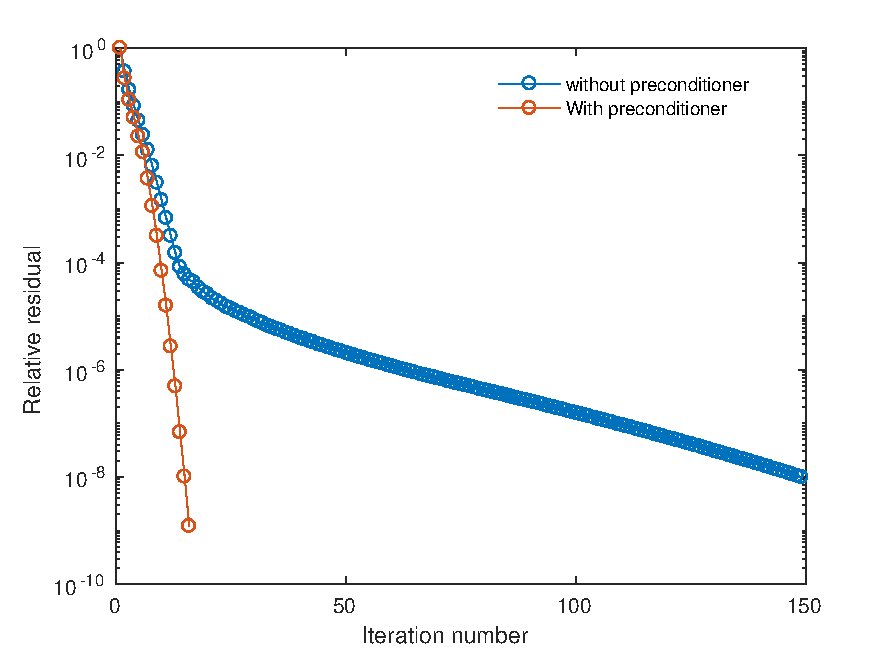
\includegraphics[scale=0.5]{figs/PrecondDirichletHelmSegPDF}
	\caption{Number of iteration in the resolution of the single layer integral equation with a mesh of size $N \approx 3700$, $L = 800 \lambda$.}
	\label{FigureNitHelmDirichlet}
\end{figure}
\paragraph{Flat segment, Neumann boundary condition.} We run the same numerical comparisons, this time with the precondioning operator $\left(-(\partial_x \omega)^2 - k^2 \omega^2\right)^{-1/2}$. 
\begin{table}[H]
	\begin{center}
		\begin{tabular}{|| m{4em} | m{4em} | m{4em} | m{4em} | m{4em}||} 
			\hline
			\multicolumn{1}{||c|}{ }&
			\multicolumn{2}{c|}{with Prec.}&\multicolumn{2}{c||}{without Prec.}\\
			\hline
			$L/\lambda$ & $n_{it}$& t(s) & $n_{it}$ & t(s)\\
			\hline\hline
			50 & 8 & 0.08 & 785 & 9.4\\
			\hline
			200 & 10 & 3.6 & - &  $>$ 2min\\
			\hline
			800 & 17 & 73 & - & -\\
			\hline
		\end{tabular}
	\end{center}
	\caption{Number of iteration and time needed for the numerical resolution of \eqref{Somegaalpha} using Galerkin finite elements with and without preconditioner.}
	\label{TableNitTimeHlemholtzNeumann}
\end{table}
\begin{figure}[H]
	\centering
	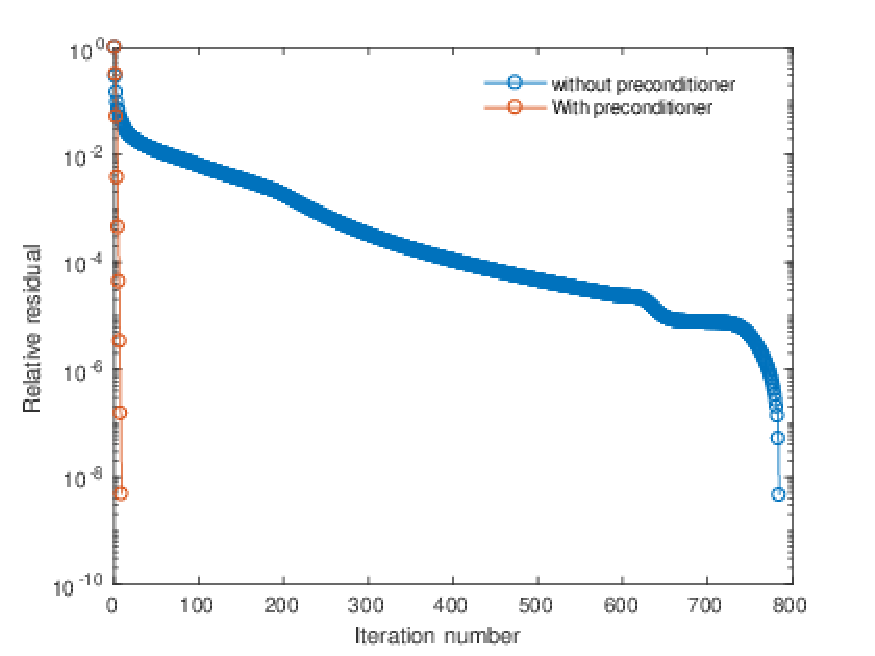
\includegraphics[scale=0.5]{figs/PrecondNeumannHelmSegPDF}
	\caption{Number of iteration in the resolution of Hypersingular integral equation with a mesh of size $N \approx 800$, $L = 50 \lambda$.}
	\label{FigureNitHelmNeumann}
\end{figure}
\paragraph{Non-flat arc.} Here, we also report numerical results when the curve is an portion of spiral (see \autoref{ArcOfSpiral}), for both boundary conditions. This shows that the preconditioning strategy is also efficient in presence of non-zero curvature. 
\begin{table}[H]
	\begin{center}
		\begin{tabular}{|| m{4em} | m{4em} | m{4em} | m{4em} | m{4em}||} 
			\hline
			\multicolumn{1}{||c|}{ }&
			\multicolumn{2}{c|}{Dirichlet}&\multicolumn{2}{c||}{Neumann}\\
			\hline
			$L/\lambda$ & $n_{it}$& t(s) & $n_{it}$ & t(s)\\
			\hline\hline
			50 & 23 & 0.6 & 785 & 9.4\\
			\hline
			200 & 27 & 9 & - &  $>$ 2min\\
			\hline
			800 & 40 & 35 & - & -\\
			\hline
		\end{tabular}
	\end{center}
	\caption{Number of iterations of the preconditioned system }
	\label{TableNitTimeHlemholtzDirSpiral}
\end{table}
\begin{figure}[H]
	\centering
	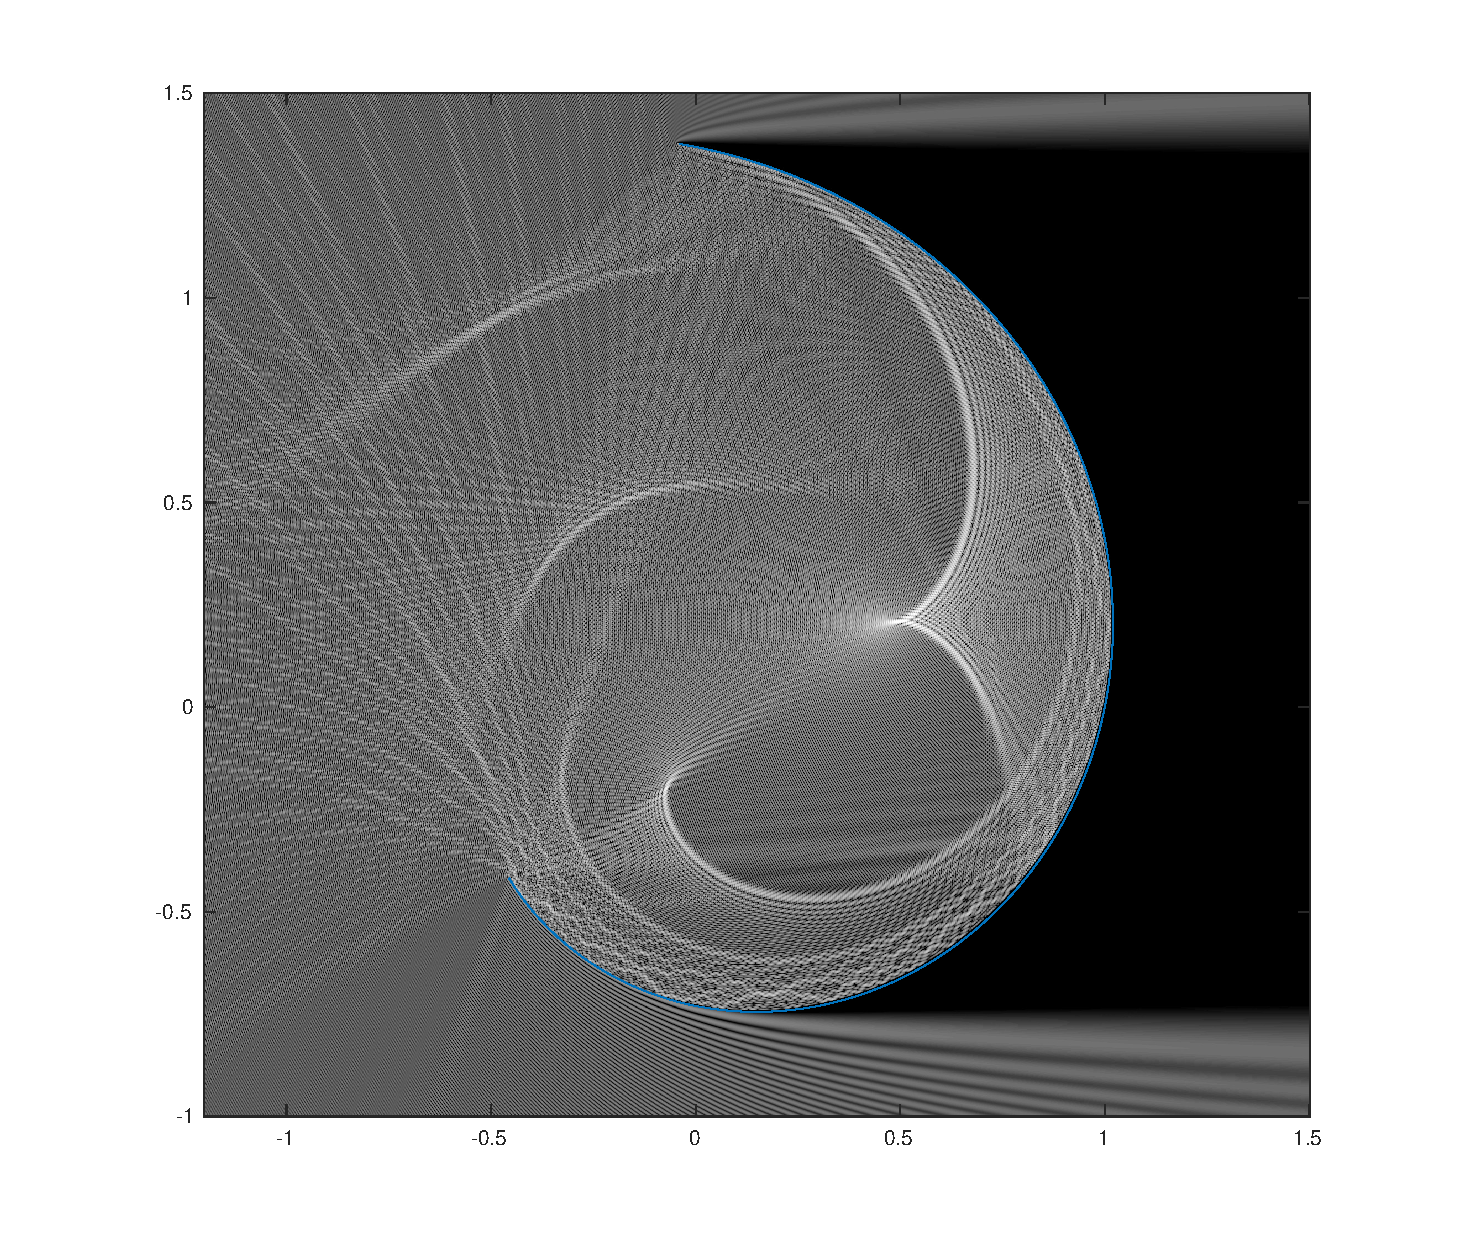
\includegraphics[width=1\linewidth]{figs/arcOfSpiral800_3}
	\caption{Sample diffraction pattern (Dirichlet boundary conditions) with left to right incidence for an arc of spiral of size $L = 800 \lambda$. After the resolution of the integral equation, the image is obtained in a few seconds.}
	\label{ArcOfSpiral}
\end{figure}
\paragraph{Comparison with the generalized Calderon relations.} As shown in \cite{bruno2012second}, $S_\omega$ and $N_\omega$ can be used efficiently as mutual preconditioners. This alternative method is also very efficient in our numerical setting (here, we use simple piecewise affine functions, whereas in \cite{bruno2012second}, spectral discretization with trigonometric polynomials is used.) We report in \autoref{TableBrunoVsSqrt} the number of iterations and computing times for the Neumann problem with an angle of incidence $\frac{\pi}{4}$ on the flat segment. The number iterations are comparable for the two methods. However, the matrix-vector product time in our method is significantly slower as it only involves sparse operators. This leads to a faster resolution of the linear system. 

\begin{table}[H]
	\begin{center}
		\begin{tabular}{|| m{4em} | m{4em} | m{4em} | m{4em} | m{4em}||} 
			\hline
			\multicolumn{1}{||c|}{ }&
			\multicolumn{2}{c|}{Calderon Prec.}&\multicolumn{2}{c||}{Square root Prec.}\\
			\hline
			$L/\lambda$ & $n_{it}$& t(s) & $n_{it}$ & t(s)\\
			\hline\hline
			50 & 14 & 0.1 & 8 & 0.1\\
			\hline
			200 & 15 & 7.5 & 11 &  3.6\\
			\hline
			800 & 16 & 130 & 15 & 70\\
			\hline
		\end{tabular}
	\end{center}
	\caption{Number of iteration and time needed for the numerical resolution of \eqref{Somegaalpha} using Galerkin finite elements with and without preconditioner.}
	\label{TableBrunoVsSqrt}
\end{table}

\section{Numerical methods}


\subsection{Galerkine setting}

\label{subsec:GalerkineSetting}

In this section, we describe and analyze the Galerkin scheme used to solve the integral equations in this work. To keep matters simple, we focus on equations \eqref{Slambda} and \eqref{Nmu} on the flat strip. The results extend to the general case using standard arguments in the theory of boundary element methods. Standard discretization on a uniform mesh with piecewise polynomial trial functions leads to very poor rates of convergences (see for example \cite[Chap. 4, ]{sauter2011boundary} and subsequent remark). Several methods have been developed to remedy this problem. One can for example enrich the trial space with special singular functions, refine the mesh near the segment tips, (h-BEM) or increase the polynomial order in the trial space. The combination of the last two methods, known as h-p BEM, can achieve an exponential rate of convergence with respect to the dimension of the trial space, see \cite{postell1990h} and references therein. Spectral methods, involving trigonometric polynomials have also been analyzed for example \cite{bruno2012second}, and some results exist for piecewise linear functions in the colocation setting \cite{costabel1988convergence}. 

Here, we describe a simple Galerkin scheme using piecewise affine functions on an adapted mesh, that is both stable and easy to implement. Our analysis shows that the usual rates of convergence one would obtain with smooth closed boundary with smooth solution, are recovered thanks to this new analytic setting. The orders of convergence are stated in \autoref{theOrdreCVDirichlet} and \autoref{theOrdreCVNeumann}. 

In what follows, we introduce a discretization of the segment $[-1,1]$ as $-1 = x_0 < x_1 < \cdots < x_N = 1$, and let $\theta_i \isdef \arccos(x_i)$. We define the parameter $h$ of the discretization as 
\[ h \isdef \min_{i=0\cdots N-1} \abs{\theta_{i+1} - \theta_{i}}.\]
In practice, one should use a mesh for which $\abs{\theta_i - \theta_{i+1}}$ is constant. This turns out to be analog to a graded mesh with the grading parameter set to $2$, that is, near the edge, the width of the $i-th$ interval is approximately $(ih)^2$. In comparison, in the h-BEM method with $p=1$ polynomial order, this would only lead to a convergence rate in $O(h)$ (cf. \cite[Theorem 1.3]{postell1990h}).

\subsubsection{Dirichlet problem}

In this section, we present the method to compute a numerical approximation of the solution $\lambda$ of \eqref{Slambda}. To achieve it, we use a variational formulation of \eqref{Somegaalpha} to compute an approximation $\alpha_h$ of $\alpha$, and set $\lambda_h = \frac{\alpha_h}{\omega}$. Let $V_h$ the Galerkin space of (discontinuous) piecewise affine functions with breakpoints at $x_i$. Let $\alpha_h$ the unique solution in $V_h$ to
\[ \duality{S_\omega \alpha_h}{\alpha_h'}_\frac{1}{\omega} = -\duality{u_D}{\alpha_h'}_\frac{1}{\omega}, \quad \forall \alpha_h' \in V_h.\]
We shall prove the following result:
\begin{The}
	If the data $u_D$ is in $T^{s+1}$ for some $-1/2 \leq s \leq 2$, then there holds:
	\[ \norm{\lambda - \lambda_h}_{\tilde{H}^{-1/2}} \leq C h^{s+1/2} \norm{u_D}_{T^{s+1}}.\]
	\label{theOrdreCVDirichlet}
\end{The}
In particular, when $u_D$ is smooth, it belongs to $T^{\infty}$ so the rate of convergence is $h^{5/2}$.
\noindent We start by proving an equivalent of Céa's lemma: 
\begin{Lem}
	\label{CeaDir}
	There exists a constant $C$ such that 
	\[\norm{\alpha - \alpha_h}_{T^{-1/2}} \leq C \inf_{{\alpha}_h' \in V_h}\norm{\alpha - {\alpha}_h'}_{T^{-1/2}}\]
	\begin{proof}
		In view of the properties of $S_\omega$ stated in \autoref{STn}, we have the equivalent norm 
		\[\norm{\alpha - \alpha_h}_{T^{-1/2}}^2 \leq C \duality{S_\omega(\alpha - \alpha_h)}{\alpha-\alpha_h}.\] 
		Since $\duality{S_\omega \alpha}{\alpha_h'} = \duality{S_\omega \alpha_h}{\alpha_h'} = -\duality{u_D}{\alpha_h'}$ for all $\alpha_h' \in V_h$, we deduce 
		\[\norm{\alpha - \alpha_h}_{T^{-1/2}}^2 \leq \duality{S_\omega (\alpha - \alpha_h)}{\alpha - \alpha'_h}, \quad \forall \alpha'_h \in V_N.\]
		By duality
		\[\norm{\alpha - \alpha_h}_{T^{-1/2}}^2 \leq C \norm{S_\omega(\alpha - \alpha_h)}_{T^{1/2}}\norm{\alpha - \alpha'_h}_{T^{-1/2}}\]
		which gives the desired result after using the continuity of $S_\omega$ from $T^{-1/2}$ to $T^{1/2}$. 
	\end{proof}
\end{Lem}
From this we can derive the rate of convergence for $\alpha_h$ to the true solution $\alpha$. We use the $L^2_\frac{1}{\omega}$ orthonormal projection $\mathbbm{P}_h$ on $V_h$, which satisfies the following properties:
\begin{Lem}
	For any function $u$, 
	\[\norm{(\textup{I} - \mathbbm{P}_h)u}_{L^2_\frac{1}{\omega}} \leq C\norm{u}_{L^{2}_\frac{1}{\omega}},\]
	\[\norm{(\textup{I} - \mathbbm{P}_h)u}_{L^2_\frac{1}{\omega}}  \leq C h^2 \norm{u}_{T_2}.\]
	\label{PhT0T2}
\end{Lem}
\noindent The proof requires the following well-known result:
\begin{Lem}
	\label{LemH2NulAuBord}
	Let $\tilde{u}$ in the Sobolev space $H^2(\theta_1,\theta_2)$,such that $\tilde{u}(\theta_1) = \tilde{u}(\theta_2) = 0$. Then there exists a constant $C$ independent of $\theta_1$ and $\theta_2$ such that 
	\[ \int_{\theta_1}^{\theta_2} \tilde{u}(\theta)^2 \leq C(\theta_1-\theta_2)^4 \int_{\theta_1}^{\theta_2} \tilde{u}''(\theta)^2 d\theta\]
\end{Lem}
\begin{proof}
	The first inequality is obvious since $\mathbbm{P}_h$ is an orthonormal projection. For the second inequality, we first write, since the orthogonal projection minimizes the $L^2_\frac{1}{\omega}$ norm,
	\begin{equation}
	\norm{I - \mathbbm{P}_h u}_{L^2_\frac{1}{\omega}} \leq \norm{I - I_h u}_{L^2_\frac{1}{\omega}},
	\label{estimProjParInterp}
	\end{equation}
	where $I_h u$ is the piecewise affine (continuous) function that matches the values of $u$ at the breakpoints $x_i$. By \autoref{thmChar}, on each interval $[x_i, x_{i+1}]$, the function $\tilde{u}(\theta) \isdef u(\cos(\theta))$ is in the Sobolev space $H^2(\theta_i,\theta_{i+1})$ so we can apply \autoref{LemH2NulAuBord}:
	\[ \int_{x_i}^{x_{i+1}} \frac{(u - I_h u)^2}{\omega} = \int_{\theta_i}^{\theta_{i+1}} (\tilde{u}- \tilde{I_h}u)^2 \leq (\theta_{i+1} - \theta_i)^4 \int_{\theta_{i}}^{\theta_{i+1}} (\tilde{u} - \tilde{I_hu})''^2. \]
	This gives
	\begin{equation}
	\int_{x_i}^{x_{i+1}} \frac{(u - I_h u)^2}{\omega} \leq 2h^4 \left(\int_{\theta_i}^{\theta_{i+1}} \tilde{u}''^2 + \int_{\theta_i}^{\theta_{i+1}} \tilde{I_h}u''^2 \right).
	\label{enCoursDePreuve}
	\end{equation}
	Before continuing, we need to establish the following result
	\begin{Lem}
		There holds 
		\[ \int_{\theta_i}^{\theta_{i+1}} \tilde{I_hu}''^2 \leq C \int_{x_i}^{x_{i+1}} \frac{u'^2}{\omega}\]
	\end{Lem}
	\begin{proof}
		The expression of $I_h u$ is given by
		\[\tilde{I_h u}(\theta) = u(x_i) + \frac{u(x_i) - u(x_{i+1})}{\cos(\theta_{i+1}) - \cos(\theta_i)} (\cos(\theta) - \cos(\theta_i)),\]
		thus
		\[\int_{\theta_i}^{\theta_{i+1}} \tilde{I_hu}''^2 = \left(\frac{u(x_i) - u(x_{i+1})}{\cos(\theta_{i+1}) - \cos(\theta_i)}\right)^2 \int_{\theta_i}^{\theta_{i+1}} \cos(\theta)^2 d\theta.\]
		We can rewrite 
		\[\left(u(x_{i+1}) - u(x_i)\right)^2 = \left( \int_{x_i}^{x_{i+1}} u'(t)dt\right)^2,\]
		and apply Cauchy-Schwarz's inequality and the variable change $t = \cos(\theta)$ to find 
		\[\left(\tilde{u}(\theta_{i+1}) - \tilde{u}(\theta_i)\right)^2 \leq \int_{x_i}^{x_{i+1}} \frac{u'^2}{\omega} \int_{\theta_i}^{\theta_{i+1}} \sin(\theta)^2 d\theta.\]
		To conclude, it remains to notice that the quantity
		\[\frac{ \int_{\theta_i}^{\theta_{i+1}} \cos(\theta)^2\int_{\theta_i}^{\theta_{i+1}} \sin(\theta)^2}{(\cos(\theta_{i+1}) - \cos(\theta_i))^2}\]
		is bounded uniformly in $(\theta_i, \theta_{i+1})$. Indeed, since $\cos$ is injective on $[0,\pi]$, the only problematic case is the limit when $\theta_i = \theta_{i+1}$. It is easy to check that this limit is $\cos(\theta_i)^2$, which is indeed uniformly bounded in $\theta_i$. 	
	\end{proof}
	\noindent We can now conclude the proof of \autoref{PhT0T2}. Summing all inequalities \eqref{enCoursDePreuve} for $i = 0, \cdots N+1$, we get 
	\[\norm{u - I_h u}_{L^2_\frac{1}{\omega}}^2 \leq Ch^4 \left( \norm{u}_{T^2}^2 + \norm{u'}_{T_0}^2\right).\]
	By \autoref{corDxT2T0}, the operator $\partial_x$ is continuous from $T^2$ to $T^0$ which gives 
	\[\norm{u - I_hu}_{L^2_\frac{1}{\omega}} \leq Ch^2 \norm{u}_{T^2}.\]
	Thanks to \eqref{estimProjParInterp}, this concludes the proof. 
\end{proof}
\noindent We obtain the following corollary by interpolation:
\begin{Cor}
	\label{interpImoinsP}
	The operator $\textup{I} - \mathbbm{P}_N$ is continuous from $L^2_\frac{1}{\omega}$ to $T^s$ for $0 \leq s \leq 2$ with
	\[\norm{(\textup{I} - \mathbbm{P}_N)u}_{L^2_\frac{1}{\omega}} \leq c h^s \norm{u}_{T^s}.\]
\end{Cor}
\noindent We can now prove \autoref{theOrdreCVDirichlet}:
\begin{proof}
	First, using \autoref{LemmaT-1/2}, one has 
	\[\norm{\lambda - \lambda_h}_{\tilde{H}^{-1/2}} \sim \norm{\alpha - \alpha_h}_{T^{-1/2}}.\]
	Moreover, if $u_D$ is in $T^{s+1}$, then $\alpha = S_\omega^{-1} u_D$ is in $T^s$ and $\norm{\alpha}_{T^s} \sim \norm{u_D}_{T^{s+1}}$. 	
	By the analog of Céa's lemma, \autoref{CeaDir}, it suffices to show that 
	\[ \norm{\alpha - \mathbbm{P}_h \alpha}_{T^{-1/2}} \leq C h^{s + 1/2} \norm{\alpha}_{T^s}.\]
	For this, we write
	\[\norm{\alpha - \mathbbm{P}_h \alpha}_{T^{-1/2}} = \inf_{\eta \in T^{1/2}, \eta \neq 0} \dfrac{(\alpha - \mathbbm{P}_h \alpha,\eta)_{\frac{1}{\omega}}}{\norm{\eta}_{T^{1/2}}}\]
	and since $\mathbbm{P}_h$ is an orthonormal projection on $L^2_\frac{1}{\omega}$, 
	\[\norm{\alpha - \mathbbm{P}_h \alpha}_{T^{-1/2}} = \inf_{\eta \in T^{1/2}, \eta \neq 0} \dfrac{(\alpha - \mathbbm{P}_N \alpha,\eta -\mathbbm{P}_h \eta )_{\frac{1}{\omega}}}{\norm{\eta}_{T^{1/2}}}.\]
	Using Cauchy-Schwarz's inequality and \autoref{interpImoinsP} ($s = \frac{1}{2}$), 
	\[\norm{\alpha - \mathbbm{P}_h \alpha}_{T^{-1/2}} \leq \dfrac{h^s \norm{\alpha}_{T^s} h^{1/2}\norm{\eta}_{T^{1/2}}}{\norm{\eta}_{T^{1/2}}} = h^{s+\frac{1}{2}} \norm{\alpha}_{T^s}.\]
\end{proof}

\subsubsection{Neumann problem}

We now turn to the numerical resolution of \eqref{Nmu}. We use a variational form for equation \eqref{Nomegabeta}, and solve it using a Galerkin method with continuous piecewise affine functions. We introduce $W_h$ the space of continuous piecewise affine functions with breakpoints at $x_i$, and we denote by $\beta_h$ the unique solution in $W_h$ to the variational equation:
\begin{equation}
\duality{N_\omega \beta_h}{\beta_h'}_{\omega} = \duality{u_N}{\beta_h'}_{\omega}, \quad \forall \beta_h' \in W_h.
\label{NomegaBetaGalerk}
\end{equation}
Then, $\mu_h = \omega \beta_h$ is the proposed approximation for $\mu$. 
We shall prove the following:
\begin{The}
	If $u_N \in U^{s-1}$, for some $\frac{1}{2} \leq s \leq 2$, there holds 
	\[\norm{\mu - \mu_h}_{\tilde{H}^{1/2}} \leq C h^{s - \frac{1}{2}}\norm{u_N}_{U^{s-1}}.\]
	\label{theOrdreCVNeumann}
\end{The}
\noindent Like before, we start with an analog of Céa's lemma:
\begin{Lem}
	There exists a constant $C$ such that
	\[\norm{\beta - \beta_h}_{U^{1/2}} \leq C \inf_{\beta'_h \in W_h} \norm{\beta - \beta'_h}_{U^{1/2}}\] 
	\label{CeaNeumann}
\end{Lem}
\noindent In a similar fashion as in the previous section, it is possible to show the following continuity properties of the interpolation operator $I_h$: 
\begin{Lem} 
	\label{U0U2,U1U2}
	There holds 
	\[ \norm{ u - I_h u}_{L^2_\omega} \leq Ch^2\norm{u}_{U^2}\]
	and
	\[\norm{u-I_h u}_{U^1} \leq Ch \norm{u}_{U^2}\]	
\end{Lem}
\begin{proof}
	We only show the first estimation, the method of proof for the second being similar. Using again \autoref{LemH2NulAuBord} on each segment $[x_i, x_{i+1}]$, one can write
	\begin{eqnarray*}
		\int_{x_i}^{x_{i+1}} \omega (u - I_h u)^2 &\leq& C  (\theta_{i+1} - \theta_i)^4 \int_{\theta_i}^{\theta_{i+1}} (Vu- VI_h u)''^2 \\
		&\leq& C h^4 \left(2\int_{\theta_i}^{\theta_{i+1}} Vu''^2 + 2\int_{\theta_i}^{\theta_{i+1}}(VI_hu)''^2\right)
	\end{eqnarray*}
	where we recall that for any function $u$, $Vu$ is defined as 
	\[Vu(\theta) = \sin(\theta)u(\cos(\theta)).\] 
	Before continuing, we need to establish the following estimate:
\begin{Lem}
	\[\int_{\theta_i}^{\theta_{i+1}} (VI_hu)''^2 \leq  C \left(\norm{u}^2_{U_2} \int_{\theta_i}^{\theta_{i+1}} \sin^2 +  \int_{x_i}^{x_{i+1}} \omega (\partial_x u)^2\right)\]
	\label{LemIntermediaire}
\end{Lem}
\begin{proof}
	Using the expression of $I_h$, one can write
	\begin{multline}
	\int_{\theta_i}^{\theta_{i+1}} (V I_hu)''^2\leq C\left(\abs{ u(x_i)}^2 \int_{\theta_i}^{\theta_{i+1}} \sin^2 \right.\\
	\left.+ \left(\frac{u(x_{i+1}) -  u(x_{i})}{\cos\theta_{i+1} - \cos\theta_i}\right)^2 \int_{\theta_i}^{\theta_{i+1}} \sin^2(1 + \cos^2)\right)
	\label{CalculIntermediaire}
	\end{multline}
	We can estimate the first term, thanks to \autoref{LemInjectionsContinues}:
	\[\abs{ u(x_i)} \leq C \norm{u}_{U^2},\]
	while for the second term, the numerator of is estimated as follows: 
	\begin{eqnarray*}
		\left(u(x_{i+1}) - u(x_i)\right)^2 &=& \left(  \int_{x_i}^{x_{i+1}} \partial_x  u\right)^2 \\
		& \leq & \int_{x_i}^{x_{i+1}} \omega (\partial_x u)^2 \int_{x_i}^{x_{i+1}} \frac{1}{\omega} \\
		&  = & \abs{\theta_{i+1} - \theta_i}\int_{x_i}^{x_{i+1}} \omega (\partial_x u)^2.
	\end{eqnarray*}
	to conclude, it remains to observe that the quantity 
	\[\frac{\abs{(\theta_{i+1} - \theta_i)} \int_{\theta_i}^{\theta_{i+1}}{\sin^2(1 + \cos^2)}}{(\cos(\theta_{i}) - \cos(\theta_{i+1}))^2}\]
	is bounded by a constant independent of $\theta_i$ and $\theta_{i+1}$. Indeed, in the limit $\theta_{i+1} \to \theta_{i}$, the fraction has the value $1 + \cos^2(\theta_i)$ 
\end{proof}
	\noindent We now plug the estimate \autoref{LemIntermediaire} in \eqref{CalculIntermediaire}, and sum over $i$:
	\[\norm{u - I_hu}^2_{L^2_\omega} \leq C h^4(\norm{u}_{U^2}^2 + \norm{u'}_{L^2_\omega}^2).\]
	This implies the claim once we use the continuity of $\partial_x$ from $U^2$ to $U^0$, cf. \autoref{corDxT2T0}.
\end{proof}
\noindent We can now prove \autoref{theOrdreCVNeumann}
\begin{proof}
	Let us denote by $\Pi_h$ the Galerkin projection operator defined by $\beta \mapsto \beta_h$. Since it is an orthogonal projection on $W_h$ with respect to the scalar product $(\beta,\beta') \isdef \duality{N_\omega \beta}{\beta'}$, it is continuous from $U^{1/2}$ to itself, so we have for any $u$ in $U^{1/2}$. 
	\[\norm{(I - \Pi_h)u}_{U^{1/2}} \leq C \norm{u}_{U^{1/2}}.\]
	We are now going to show the estimate
	\[\norm{(I - \Pi_h)u}_{U^{1/2}} \leq C h^{3/2} \norm{u}_{U^{2}}.\]
	By the analog of Céa's lemma \autoref{CeaNeumann}, one has $\norm{(I-\Pi_h)u}_{U^{1/2}} \leq \norm{(I - I_h) u}_{U^{1/2}}$. By interpolation, this norm satisfies
	\[\norm{(I - I_h)u}_{U^{1/2}} \leq C \sqrt{\norm{(I - I_h)u}_{U^{0}}}\sqrt{\norm{(I - I_h)u}_{U^{1}}},\]
	which yields, applying \autoref{U0U2,U1U2},
	\[\norm{(I - I_h)u}_{U^{1/2}} \leq C h^{3/2} \norm{u}_{U^2}.\]
	By interpolation, for all $s \in [1/2,2]$, we get
	\[\norm{(I - \Pi_h)u}_{U^{1/2}} \leq C h^{s - 1/2} \norm{u}_{U^s}.\]
	In view of \autoref{lemU12H12}, we have $\norm{\mu - \mu_h}_{\tilde{H}^{1/2}} \sim \norm{(I - \Pi_h)\beta}_{U^{1/2}}$. Moreover, since $N_\omega$ is a continuous bijection from $U^{s+1}$ to $U^s$ for all $s$, there holds
	\[\norm{\beta}_{U^s} = \norm{N_\omega^{-1} u_N}_{U^s} = \norm{u_N}_{U^{s-1}}.\]
	Consequently, 
	\[\norm{\mu - \mu_h}_{\tilde{H}^{1/2}} \leq  C\norm{(I - \Pi_h)\beta}_{U^{1/2}} \leq C h^{s - 1/2} \norm{\beta}_{U^s} \leq C h^{s - 1/2} \norm{u_N}_{U^{s-1}}.\]
\end{proof}

\subsubsection{Numerical quadratures and compression method}

\paragraph{Weakly singular kernels.} To compute the elements of the matrix of the operators which kernel have a weak singularity, we use Gaussian quadratures for the weights $\frac{1}{\omega}$ and $\omega$, with $3$ points on each segment. As a result, we obtain a vector $(x_k)$ of $3N$ points in $\R^2$ and a vector $(w_k)$ of $3N$ quadrature weights. If $p$ stands for the weight ($1/\omega$ or $\omega$), then quantities of the form $\int_\Gamma \int_\Gamma  p(x)p(y)\phi_i(x) G_k(x,y) \phi_j(y)$, are approximated by
\begin{equation}
\label{approxDoubleIntegral}
	\int_\Gamma \int_\Gamma   p(x)p(y)\phi_i(x) G_k(x,y) \phi_j(y) \approx \sum_{k = 1}^N w_k \phi_i(x_k) \sum_{l = 1}^N  w_l G(x_k,x_l) \phi_j(x_l).
\end{equation}
Since the kernel $G_k$ is singular, we must correct the previous formula when $x_k$ and $x_l$ are close from each other. This is done by the following method. For each segment $I_n$ in the mesh, we find the subset $(x_k')$of the points $x_k$ that are closer than a fixed threshold from $I_n$. For those points, we compute more accurately the integral 
\[ \int_{I_n} p(y)G_k(x_k,y) \phi_j(y),\]
by any method at our disposal (variable change, substraction of the singularity...). The second integral is then approximated using the previous quadrature. 
Note that in this framework, the addition of the wait $p$ requires only minor modification over a standard BEM code. Basically, one only needs to compute numerical quadratures for the weight $p$, for which open source routines are available, and implement a method to compute the close integrals with the weight $p$. Note that using the variable change $x = \cos(\theta)$, the weight disappears and the only singularity left is that of $G_k$. 

\paragraph{Hypersingular operator.} Although the weighted hypersingular $N_{k,\omega}$ operator has a non-integrable kernel, the formulawe have the formula
\[\duality{N_{k,\omega} \beta}{\beta'}_\omega = \duality{S_{k,\omega}\left(\omega \partial_x \omega \right)u}{\left(\omega \partial_x \omega \right) v}_\frac{1}{\omega} - k^2 \duality{S_\omega \omega^2 u}{\omega^2 v}_\frac{1}{\omega}.\]
This only involves weakly singular kernels and is thus treated by the previous method. 

\paragraph{Compression method} The rhs of \eqref{approxDoubleIntegral} is the scalar product of a vector with a discrete convolution. To accelerate the computation and to avoid assembling the full matrix $(G_k(x_k,x_l))$, we use \toDo{Citer EBD alors que pas encore accepté ?}. 

\subsection{Preconditioning the linear systems}

For an operator $A$, let us denote by $\left[A\right]_p$ the Galerkine matrix of the operator for the weight $p(x)$. When the operator $BA$ is a compact perturbation of the identity (either in $T^s$ or $U^s$) then, following \cite{steinbach1998construction}, we precondition the linear system $\left[A\right]_p x = y$ by the matrix $\left[I\right]^{-1}_p \left[B\right]_p \left[I\right]_p^{-1}$. If $B$ is the inverse of a local operator $C$, then it is easier to compute $\left[C\right]_p$. This time, the good choice for the preconditioner is $\left[C\right]_p^{-1}$. When testing the pair $S_{k,\omega}, N_{k,\omega}$ as mutual preconditioner, the operator $S_{k,\omega}N_{k,\omega}$ is discretized as $\left[I_d\right]_\frac{1}{\omega}^{-1} \left[S_{k,\omega}\right]_\frac{1}{\omega}\left[I_d\right]_{\omega}^{-1}\left[N_{k,\omega}\right]_\omega$, yielding very satisfactory results. 

The preconditioners introduced in this work are in the form of square roots of local operators. More precisely, we introduced two preconditioners $P_1$ and $P_2$ with 
\begin{eqnarray*}
	P_1(k) &=& \left(-(\omega \partial_x)^2 - k^2 \omega^2\right)^{1/2}\\
	P_2(k) &=& \left(-(\partial_x \omega)^2 - k^2 \omega^2 \right)^{-1/2}
\end{eqnarray*}
For the second equation, we rewrite 
\[P_2(k) = \left(-(\partial_x \omega)^2 - k^2 \omega^2 \right)^{-1} \left(-(\partial_x \omega)^2 - k^2 \omega^2 \right)^{1/2},\]
which brings us back to computing the square root of a sparse matrix. When the frequency is $0$, we use the method exposed in \cite{hale2008computing}. When the frequency is non-zero, the previous method fails since the spectrum of the matrix contains negative values. In \cite{antoine2007generalized}, a method involving a Padé approximation of the square root, with a rotated branch cut, is used to compute the matrix of an operator of the form $\sqrt{X - k^2 I_d}$ where $X$ is a positive definite operator. This method gives excellent results in our context when using $X = -(\partial \omega_x)^2 + k^2 \left(I_d - \omega^2\right)$. 

\section{Conclu}

Résumé de ce qu'on a fait, du lien qu'on a fait. Ouverture sur les singularités de type coin puis 3D. Beaucoup plus compliqué car pas de relations analytiques qui nous aident. 
Expliquer la beauté de l'approche numérique avec un poids. On propose le préconditioneur avec un test numérique ? 

Possible analyse pseudo-diff ? En reparler ? Lien avec Antoine et Darbas. 
	
\appendix
\section{Commutation of $N_\omega$ and $(\partial_x \omega)^2 + k^2\omega^2$}
\label{ann:commut}
\begin{Lem}
	\label{dxSomega2=Somegadxomega}
	For any $\phi$, there holds 
	\[\partial_x S_\omega \omega^2 \phi = S_\omega \omega \partial_x \omega \phi.\]
\end{Lem}
\begin{proof}
	In our context, the largest space encountered is $U^{- \infty}$ (As a consequence of \autoref{LemInjectionsContinues}) so we shall show that this identity holds in that space.
	For any $s$, by \autoref{omega2continuUsTs}, $\omega^2$ is a continuous operator from $U^s$ to $T^s$, $S_\omega$ is continuous from $T^s$ to $T^{s+1}$ and $\partial_x$ is continuous from $T^{s+1}$ to $U^s$ by \autoref{derivations}. Therefore, the left operator is continuous from $U^s$ to $U^s$. Similarly, the right operator is continuous from $U^{s}$ to $U^s$ for all $s$. If we fix $\phi \in U^{s}$ for some $s$, \autoref{densite} ensures that there exists a sequence $\phi_N$ in $U^{\infty}$ converging to $\phi$ in $U^{s}$. It is thus sufficient to check the identity for $\phi = U_n$. For $n \geq 1$, 
	\begin{eqnarray}
		\partial_x S_\omega \omega^2 U_n &=& \partial_x S_\omega \left(\frac{T_{n} - T_{n+2}}{2}\right)\\
		&=& \partial_x\left(\frac{T_{n}}{4n} - \frac{T_{n+2}}{4(n+2)} \right)\\
		&=& \frac{U_{n-1} - U_{n+1}}{4}\\
		&=& -\frac{T_{n+1}}{2}.
	\end{eqnarray}
	One can check that the result also holds for $n = 0$. On the other hand, for all $n$, 
	\begin{eqnarray}
		S_\omega \omega \partial_x \omega U_n &=&-(n+1) S_\omega T_{n+1}\\
		&=& -\frac{1}{2}T_{n+1}
	\end{eqnarray}
	which proves the result. 
\end{proof}
We now turn to the proof of the theorem. To ease the computations, we take some notations: let $\Delta_\omega \isdef (\omega \partial_x)^2$, $\Delta_\omega^T \isdef (\partial_x \omega)^2$,  $N_\omega \isdef N_{k,\omega}$, and $S_\omega \isdef S_{k,\omega}$. Using, equation \eqref{NkenfonctiondeSk} we can write 
\[N_\omega = -\partial_x S_\omega \omega \partial_x \omega - k^2 S_\omega \omega^2.\]
To show that $N_\omega$ and $\Delta_\omega^T + k^2\omega^2$ commute, we compute their commutator $C$ and show that it is null. 
We have 
\begin{eqnarray*}
	C &\isdef& N_\omega \Delta_\omega^T - \Delta_\omega^T N_\omega + k^2N_\omega \omega^2 - k^2 \omega^2 N_\omega \\
	&=& -\partial_x S_\omega \Delta_\omega \omega \partial_x \omega  - k^2 S_\omega \omega^2 \Delta_\omega^T \\
	&& + \partial_x \Delta_\omega S_\omega \omega \partial_x \omega + k^2 \Delta_\omega^T S_\omega \omega^2 \\
	&& - k^2 \partial_x S_\omega \omega \partial_x \omega^3 - k^4 S_\omega \omega^4 \\
	&& + k^2 \omega^2 \partial_x S_\omega \omega \partial_x \omega + k^4 \omega^2 S_\omega \omega^2
\end{eqnarray*}
where each term in the r.h.s. of the first equality gives rise to a line in the second. We rearrange the terms as follows:
\begin{eqnarray*}
	C &=& \partial_x (\Delta_\omega S_\omega - S_\omega \Delta_\omega) \omega \partial_x \omega - k^2 \partial_x S_\omega \omega \partial_x \omega^3 + k^2 \omega^2 \partial_x S_\omega \omega\partial_x \omega\\	
	&& + k^4 (\omega^2 S_\omega - S_\omega \omega^2) \omega^2\\
	&& + k^2(\Delta_\omega^T S_\omega \omega^2 - S_\omega \omega^2 \Delta_\omega^T)
\end{eqnarray*}
For the first term, we inject the commutation shown in \autoref{Commutations}. For the last line, we use the following identities: 
\[ \Delta_\omega^T = \Delta_\omega - 2x \partial_x - 1\]
\[ \omega^2 \Delta_\omega^T = \Delta_\omega \omega^2 + \omega^2 + 2 \omega x \partial_x \omega\]
Let $D = \frac{C}{k^2}$, 
\begin{eqnarray*}
	D &=& \partial_x S_\omega \omega (\omega^2\partial_x - \partial_x \omega^2) \omega  + (\omega^2 \partial_x - \partial_x \omega^2)S_\omega \omega \partial_x \omega\\
	&&+ k^2(\omega^2 S_\omega - S_\omega \omega^2) \omega^2\\
	&&+ (\Delta_\omega - 2x \partial_x - 1)S_\omega \omega^2 - S_\omega(\Delta_\omega \omega^2 + \omega^2 + 2\omega x \partial_x \omega) 
\end{eqnarray*}
We use $\omega^2 \partial_x - \partial_x \omega^2 = 2x$, and the relation $\partial_x S \omega^2 = S_\omega \omega \partial_x \omega$ to get
\begin{eqnarray*}
	D &=& 2 S_\omega \omega \partial_x x\omega + 2 x S_\omega  \omega \partial_x \omega \\
	&& + \left(k^2(\omega^2 S_\omega - S_\omega \omega^2) + \Delta_\omega S_\omega - S_\omega \Delta_\omega \right)\omega^2\\
	&& - 2 S_\omega \omega^2 - 2 x  S_\omega \omega \partial_x \omega - 2 S_\omega \omega x \partial_x \omega.
\end{eqnarray*}
Using again the commutation shown in \autoref{Commutations}, we are left with 
\begin{eqnarray*}
	D &=&  2 S_\omega \omega (\partial_x x - x \partial_x) \omega - 2 S_\omega \omega^2
\end{eqnarray*}
This is null since $\partial_x x - x \partial_x = 1$. 


\section{Proof of \autoref{the:ParametrixNkomega}}
\label{ParametrixNkomega}
From equation \eqref{NkenfonctiondeSk}, we can deduce the following formula for the weighted operator:
\begin{equation}
\label{developNkomega}
N_{k,\omega} = - \partial_x S_{k,\omega} \omega \partial_x \omega - k^2 S_{k,\omega} \omega^2
\end{equation}
If we define $L_n \isdef - \partial_x O_{n+2} \omega \partial_x \omega$, then using the mapping properties of $\partial_x$ and $\omega\partial_x\omega$ given by \autoref{derivations}, and since, by \autoref{orderOfOn}, $O_{n+2}$ is of order $n+2$ in the scale $T^s$, we deduce that $L_n$ is of order $n$ in the scale $U^s$. 
The expansion obtained for the weighted single-layer operator in \autoref{developpementHankel} yields the following expansion for $N_{k,\omega}$. 
\begin{Lem}
	\[N_{k,\omega} = N_\omega + k^2 \left( -\frac{L_1}{4}- S_\omega \omega^2 \right) + U_3\]
\end{Lem}
\noindent As a consequence, $N_{k,\omega}$ is an operator of order $-1$ in the scale $U^s$. 
Using equation \eqref{developNkomega}, we have the following expression:
\[N_{k,\omega}^2 = N_\omega^2 - k^2\left( \frac{L_1 N_\omega + N_\omega L_1}{4} + N_\omega S_\omega \omega^2 + S_\omega \omega^2 N_\omega\right) + U_2.\]
We have proved in
By definition, $L_1 = -\partial_x O_3 \omega \partial_x \omega$, while $N_\omega = - \partial_x S_\omega \omega \partial_x \omega$, thus
\[L_1 N_\omega = \partial_x (O_3 (\omega \partial_x)^2 S_\omega ) \omega \partial_x \omega.\]
Moreover, 
\[N_\omega L_1 =  \partial_x (S_\omega (\omega \partial_x)^2 O_3  ) \omega \partial_x \omega.\]
Adding these two inequalities and using \autoref{LemSwDeltaO3}, we get 
\[\frac{L_1 N_\omega + N_\omega L_1}{4} =\partial_x ( S_\omega \omega^2 S_\omega ) \omega \partial_x \omega + U_2.\]
Here again, we use the formula $\partial_x S_\omega \omega^2 = S_\omega \omega \partial_x \omega$, which yields
\[\frac{L_1 N_\omega + N_\omega L_1}{4} = S_\omega \omega \partial_x \omega \partial_x S_\omega \omega^2 = \left(-\frac{I_d}{4} + T_\infty\right)\omega^2 .\]
Since $\omega^2$ is continuous from $U^s$ to $T^s$, and using the injections $T^s\subset U^s$, any operator of the form $R \omega^2$ is smoothing in the scale $U^s$ as soon as $R$ is smoothing in the scale $T^s$. Therefore, 
\[\frac{L_1 N_\omega + N_\omega L_1}{4} = -\frac{\omega^2}{4} + U_\infty.\]
Moreover, we have
\begin{eqnarray*}
	S_\omega \omega^2 N_\omega &=& -S_\omega \omega^2 \partial_x S_\omega \omega \partial_x \omega\\
	&=& -S_\omega \omega^2 \partial_x^2 S_\omega \omega^2
\end{eqnarray*}
using again \autoref{dxSomega2=Somegadxomega}. Since $\omega^2 \partial_x ^2 = (\omega \partial_x)^2 + x \partial_x$, we get
\begin{eqnarray*}
	S_\omega \omega^2 N_\omega &=& \frac{\omega^2}{4} - S_\omega x \partial_x S_\omega \omega^2 + U_\infty
\end{eqnarray*}
Futhermore, 
\begin{eqnarray*}
	N_\omega S_\omega \omega^2 &=& -\partial_x S_\omega \omega \partial_x \omega S_\omega \omega^2.
\end{eqnarray*}
We use $\omega \partial_x \omega = \omega^2 \partial_x - x$:
\begin{eqnarray*}
	N_\omega S_\omega \omega^2 &=& -\partial_x S_\omega \omega^2 \partial_x S_\omega \omega^2 + \partial_x S_\omega x S_\omega \omega^2\\
	&=& \frac{\omega^2}{4} + \partial_x S_\omega x S_\omega \omega^2 
\end{eqnarray*}
Thus, 
\begin{eqnarray*}
	S_\omega \omega^2 N_\omega + N_\omega S_\omega \omega^2 &=& \frac{\omega^2}{2} + \left(\partial_x S_\omega xS_\omega \omega^2  - S_\omega x \partial_x  S_\omega \omega^2 \right)+ U_\infty.
\end{eqnarray*}
We are done if we prove that the operator in parenthesis is of order $2$ in the scale $U^s$. For this, we may compute the action of each one of them on $U_n$. Using the various identities at our disposal, we obtain on the on hand for $n\geq 2$ 
\[\partial_x S_\omega x S_\omega \omega^2 U_n = -\frac{T_{n+2}}{8(n+2)} -\frac{T_n}{8(n+2)} +  \frac{U_{n} + U_{n-2}}{8n(n+2)}. \]
and on the other hand
\[S_\omega x \partial_x S_\omega \omega^2 U_n = -\frac{T_{n+2}}{8(n+2)} - \frac{T_n}{8n}.\]
After substracting, this gives the rather surprising identity identity
\[\left(\partial_x S_\omega xS_\omega \omega^2  - S_\omega x \partial_x  S_\omega \omega^2 \right)U_n = \frac{U_n}{4n(n+2)}\]
which of course proves our claim.

\section{Suggestion de découpage}

J'y ai un tout petit peu réfléchi : 
\begin{itemize}
	\item[-] Les analyses pseudo-diffs des espaces $T^s$, bien qu'intéressantes, sont trop longues et ne se justifient pas vraiment dans le simple but de faire une méthode numérique. 
	\item[-] La méthode de Galerkine est bien analysée et nouvelle (à ma connaissance) mais n'est pas vraiment essentielle pour le message. 
\end{itemize}
Je pense qu'on pourrait envisager 3 articles. 
Un très concis sur la méthode numérique en elle-même. Utiliser le minimum d'info pour k=0, donner les inverses exacts, prouver la commutation des opérateurs pour k non nul, puis balancer les préconditionneurs, et mettre les figures. 

Un article un peu à part sur la méthode de Galerkine, et tous les aspects numériques (bcp moins d'impact)

Un article (peut-être juste sur arxiv ?) sur les espaces $T^s$ et $U^s$, qui donne toutes les justifications théoriques. (une sorte de version étendue de cet article.)


%	\section{Order of the operators $O_n$}
%	\label{orderOn}
%	
%	\begin{Lem}
%		\label{lemPseudoDiffOn}
%		For all $n \geq 1$, there exists a function $o_n : \N^2 \to \R$ satisfying the following conditions 
%		\begin{itemize} \item[(i)]\itemequation[sumDefiningOn]{}{$	\forall k \in \Z, \quad O_n T_k = \displaystyle\sum_{i = -\infty}^{+\infty} o_n(k,i)T_{k-i}$}{}
%			\item[(ii)] \itemequation[conditionon]{}{$	\forall \alpha, \in \N, \forall  i,k  \in \Z, \quad  \abs{\Delta_k^\alpha o_n(k,i)} \leq C_{n,\alpha,\beta} (1 + k^2)^{-n - \alpha}$}{} 
%			\item[(iii)]\itemequation[conditionon]{}{$\forall i,k \in \Z, \quad \abs{i} \geq  n \implies o_n(k,i) = 0$}{}
%		\end{itemize}
%		where $\Delta_i$ and $\Delta_k$ represent the discrete derivation operator in the variables $i$ and $k$ respectively, e.g. 
%		\[ \Delta_i o_n(k,i) = o_n(k,i+1) - o_n(k,i),\]
%		and $\Delta_i^\alpha$ denotes the $\alpha$-th iterate of $\Delta_i$. We use the convention $T_k \isdef T_{\abs{k}}$ for $k \in \Z$. 
%	\end{Lem}
%	\begin{proof}
%		We shall prove this by induction. First for $n = 1$, $O_1 = 2\pi S_\omega$, and we simply have $o_1(k,i) = \delta_{i = 0} s_k$ where $s_k$ are the eigenvalues of $S_\omega$ defined in \autoref{STn}. Obviously, $o_1$ satisfies all the requirements. Second, notice that for $n \geq 1$, 
%		\[O_{n+1} = x O_n - O_n x,\]
%		which combined with the identity 
%		\[x T_n = \dfrac{T_{n-1} + T_{n+1}}{2}\]
%		valid for all $n \in \Z$, implies
%		\[O_{n+1}T_k = \sum_{i= -\infty}^{+\infty} o_n(k,i) \dfrac{T_{k - i + 1} + T_{k _-i- 1}}{2} - \frac{1}{2} O_n T_{k+1} - \frac{1}{2} O_n T_{k - 1}.\]
%		By the recurrence assumption (i), this implies 
%		\begin{eqnarray*}
%			O_{n+1}T_k &=& \frac{1}{2} \sum_{-\infty}^{+ \infty}\left(o_n(k,i-1) - o_n(k+1,i - 1)\right) T_{k - i} \\
%			&&+ \frac{1}{2} \sum_{-\infty}^{+ \infty}\left(o_n(k,i+1) - o_n(k-1,i + 1)\right) T_{k - i}.
%		\end{eqnarray*}
%		Thus, condition (i) is satisfied with 
%		\[o_{n+1}(k,i) \isdef \frac{\left(o_n(k,i-1) - o_n(k+1,i-1) + o_n(k,i+1) - o_n(k-1,i+1)\right)}{2}.\]
%		If $\abs{i} \geq n+1$ then by triangular inequality $\abs{i-1} \geq n$ and $\abs{i+1} \geq n$ so all terms in the rhs are null by the assumption (iii), which shows that (iii) also holds for $o_{n+1}$. Finally, the assumption (ii) is easily checked for $o_{n+1}$ once we write 
%		\[ o_{n+1}(k,i) = \frac{- \Delta_ko_n(k,i-1) + \Delta_ko_n(k-1,i+1)}{2}.\]
%	\end{proof}
%	
%	
%	\begin{Lem}
%		\label{orderOfOn}
%		The operator $O_n$ is of order $n$. 
%	\end{Lem}
%	\begin{proof}
%		Since the sum in \eqref{sumDefiningOn} is finite, by linearity, it is sufficient to show that the operator $O^i_n$ defined by 
%		\[ \forall k \in \Z, \quad  O^i_n T_k = o_n(k,i) T_{k-i} \]
%		is of order $n$. We treat the case $i > 0$, the opposite case being analogous. Let $u \in T^s$ for some $s$, there holds 
%		\[ O^i_n u = \sum_{k = 0}^{+ \infty} o_n(k + i,i)\hat{u}_{k + i}T_k + \sum_{k = 0}^{i} o_n(i - k,i) \hat{u}_{i - k}T_k.\]
%		We let $Vu$ and $Ru$ respectively the two terms of the rhs. Obviously, $R$ is a smoothing operator with
%		\[ \norm{Ru}_{T^{s + n}} \leq (1 + i)^{n} \norm{u}_{T^s}.\]
%		Now, for all $k \in \N$ let
%		\[\hat{v}_k \isdef o_n(i + k,i) \hat{u}_{i + k}.\]
%		Applying Peetre's inequality, one has
%		\[(1 + k^2)^{n + s}\abs{\hat{v}_k}^2 \leq C \left(1 + i^2\right)^{\abs{n + s}}\left(1 + (i + k)^2\right)^{n + s} \abs{o_n(k + i,i)}^2 \abs{\hat{u}_{k+i}}^2.\]
%		the condition (ii) in \autoref{lemPseudoDiffOn} with $\alpha = \beta = 0$ yields
%		\[\abs{o_n(k+i,i)}^2 \leq C\left(1 + (k+i)\right)^{-2n} \leq 2C \left(1 + (k+i)^2\right)^{-n}.\]
%		Therefore, $\norm{V u}_{T^{s + n}} \leq C(1 + i)^{\abs{n + s}} \norm{u}_{T^s}$ which concludes the proof. 
%	\end{proof}

	
	
	
	
	
	
	
	
	
	\bibliographystyle{plain}
	\IfFileExists{biblio.bib}{\bibliography{biblio}}{\bibliography{/home/martin/Thesis/Biblio/biblio}}
	
	
\end{document}


